\documentclass[12pt]{article}\usepackage[]{graphicx}\usepackage[]{color}
%% maxwidth is the original width if it is less than linewidth
%% otherwise use linewidth (to make sure the graphics do not exceed the margin)
\makeatletter
\def\maxwidth{ %
  \ifdim\Gin@nat@width>\linewidth
    \linewidth
  \else
    \Gin@nat@width
  \fi
}
\makeatother

\definecolor{fgcolor}{rgb}{0.345, 0.345, 0.345}
\newcommand{\hlnum}[1]{\textcolor[rgb]{0.686,0.059,0.569}{#1}}%
\newcommand{\hlstr}[1]{\textcolor[rgb]{0.192,0.494,0.8}{#1}}%
\newcommand{\hlcom}[1]{\textcolor[rgb]{0.678,0.584,0.686}{\textit{#1}}}%
\newcommand{\hlopt}[1]{\textcolor[rgb]{0,0,0}{#1}}%
\newcommand{\hlstd}[1]{\textcolor[rgb]{0.345,0.345,0.345}{#1}}%
\newcommand{\hlkwa}[1]{\textcolor[rgb]{0.161,0.373,0.58}{\textbf{#1}}}%
\newcommand{\hlkwb}[1]{\textcolor[rgb]{0.69,0.353,0.396}{#1}}%
\newcommand{\hlkwc}[1]{\textcolor[rgb]{0.333,0.667,0.333}{#1}}%
\newcommand{\hlkwd}[1]{\textcolor[rgb]{0.737,0.353,0.396}{\textbf{#1}}}%

\usepackage{framed}
\makeatletter
\newenvironment{kframe}{%
 \def\at@end@of@kframe{}%
 \ifinner\ifhmode%
  \def\at@end@of@kframe{\end{minipage}}%
  \begin{minipage}{\columnwidth}%
 \fi\fi%
 \def\FrameCommand##1{\hskip\@totalleftmargin \hskip-\fboxsep
 \colorbox{shadecolor}{##1}\hskip-\fboxsep
     % There is no \\@totalrightmargin, so:
     \hskip-\linewidth \hskip-\@totalleftmargin \hskip\columnwidth}%
 \MakeFramed {\advance\hsize-\width
   \@totalleftmargin\z@ \linewidth\hsize
   \@setminipage}}%
 {\par\unskip\endMakeFramed%
 \at@end@of@kframe}
\makeatother

\definecolor{shadecolor}{rgb}{.97, .97, .97}
\definecolor{messagecolor}{rgb}{0, 0, 0}
\definecolor{warningcolor}{rgb}{1, 0, 1}
\definecolor{errorcolor}{rgb}{1, 0, 0}
\newenvironment{knitrout}{}{} % an empty environment to be redefined in TeX

\usepackage{alltt}
\usepackage{amsmath}
\usepackage{amsthm}
\usepackage{graphicx,psfrag,epsf}
\usepackage{enumerate}
\usepackage{booktabs}
%\usepackage{natbib}
\RequirePackage[natbibapa]{apacite}

%\pdfminorversion=4
% NOTE: To produce blinded version, replace "0" with "1" below.
\newcommand{\blind}{0}

% DON'T change margins - should be 1 inch all around.
\addtolength{\oddsidemargin}{-.7in}%
\addtolength{\evensidemargin}{-.5in}%
\addtolength{\textwidth}{1in}%
\addtolength{\textheight}{1.3in}%
\addtolength{\topmargin}{-.8in}%

\usepackage{float}    % for fig.pos='H'
\usepackage{rotfloat} % for sidewaysfigure

\usepackage[textwidth=1in, textsize=tiny]{todonotes}
%\usepackage[disable]{todonotes}

\newtheorem{thm}{Theorem}
\newtheorem{lem}{Lemma}

\newcommand{\Prob}{\text{Pr}}
\newcommand{\E}{\text{E}}
\newcommand{\Cov}{\text{Cov}}
\newcommand{\corr}{\text{corr}}
\newcommand{\Var}{\text{Var}}
\newcommand{\iid}{\stackrel{\text{iid}}{\sim}}
\newcommand{\tr}{\text{tr}}
\newcommand{\bm}{\mathbf}
\newcommand{\bs}{\boldsymbol}
\IfFileExists{upquote.sty}{\usepackage{upquote}}{}
\begin{document}

\def\spacingset#1{\renewcommand{\baselinestretch}%
{#1}\small\normalsize} \spacingset{1}


%%%%%%%%%%%%%%%%%%%%%%%%%%%%%%%%%%%%%%%%%%%%%%%%%%%%%%%%%%%%%%%%%%%%%%%%%%%%%%

\if0\blind
{
  \title{\bf Small sample methods for cluster-robust variance estimation and hypothesis testing in fixed-effect models}
  \author{\\James E. Pustejovsky\thanks{
    The authors thank Dan Knopf for helpful discussions about the linear algebra behind the cluster-robust variance estimator. Coady Wing,...}\hspace{.2cm}\\
    Department of Educational Psychology \\ 
    University of Texas at Austin\\ \\
    and \\ \\
    Elizabeth Tipton \\
    Department of Human Development \\ 
    Teachers College, Columbia University}
  \maketitle
} \fi

\if1\blind
{
  \bigskip
  \bigskip
  \bigskip
  \begin{center}
    {\LARGE\bf Small sample methods for cluster-robust variance estimation and hypothesis testing in fixed-effect models}
\end{center}
  \medskip
} \fi

\bigskip
\begin{abstract}
The text of your abstract.  200 or fewer words.
\end{abstract}

\noindent%
{\it Keywords:}  3 to 6 keywords, that do not appear in the title
\vfill

\newpage
\spacingset{1.45} % DON'T change the spacing!

\section{INTRODUCTION}
\label{sec:intro}

In a wide array of economic analyses, interest centers on the parameters of linear regression models, estimated by ordinary or weighted least squares (OLS/WLS) from a sample of units that are correlated. 
Correlation among units may arise from the sampling of aggregate units (e.g., countries, districts, villages), each of which contains multiple observations; from repeated measurement of an outcome on a common set of units, as in panel data; or from model mis-specification, as in analysis of regression discontinuity designs \citep{Lee2008regression}. 
A common approach to inference in these settings is to use a cluster-robust variance estimator \citep[CRVE;][]{Arellano1987computing, Liang1986longitudinal, white1984asymptotic}.
The advantage of CRVEs is that they produce consistent standard errors and test statistics without imposing strong parametric assumptions about the dependence structure of the errors in the model.
Instead, the method relies on the relatively weaker assumption that units can be grouped into clusters that are mutually independent. 
CRVEs are an extension to another economic mainstay, heteroscedasticity-robust variance estimators \citep{eicker1967limit, Huber1967behavior, White1980heteroskedasticity}, which is used to account for non-constant variance in regression models with independent errors.
In the past decade, use of CRVE has become standard practice for applied micro-economic analysis, as evidenced by coverage in major textbooks and review articles \citep[e.g.,][]{Wooldridge2010econometric, Angrist2009mostly, Cameron2015practitioners}.

For example, consider a study of the effects on employment outcomes of several state-level policy shifts, where the policies were implemented at different time-points in each state. 
In a difference-in-differences analysis, the policy effects would be parameterized in a regression model that includes indicator variables for each policy shift, demographic controls, and fixed effects for states and time-periods in order to control for unobserved confounding in each of these dimensions. 
The model could be estimated by OLS, with the fixed effects included as indicator variables; more commonly, the effects of the policy indicators would be estimated after absorbing the fixed effects, a computational technique that is also known as the fixed effects or within transformation \citep{Wooldridge2010econometric}. 
Standard errors would then be clustered by state to account for dependence in the residual errors from a given state, and these clustered standard errors would be used to test hypotheses regarding each policy (i.e., a t-test) or across policies (i.e., an F-test).
The need to cluster the standard errors by state, even when including state fixed effects, was highlighted by \citet{Bertrand2004how}, who showed that to do otherwise can lead to inappropriately small standard errors and hypothesis tests with incorrect rejection rates. 

The consistency properties of CRVEs are asymptotic in the number of independent clusters \citep{Wooldridge2003cluster}.\footnote{Working in a panel data setting, \citet{Hansen2007asymptotic} and \citet{Donald2007inference} identified conditions under which cluster-robust test statistics converge to a limiting $t$-distribution as the number of measurement occasions increases, holding the number of independent units fixed.}
Recent methodological work has demonstrated that CRVEs can be biased downward and associated hypothesis tests can have Type-I error rates considerably in excess of nominal levels, when based on samples with only a small or moderate number of clusters \citep[e.g.,][]{Webb2013wild}.
\citet{Cameron2015practitioners} provide a thorough review of this literature, including a discussion of current practice, possible solutions, and open problems. 
In particular, they demonstrate that small-sample corrections for t-tests implemented in common software packages such as Stata and SAS do not provide adequate control of Type-I error. 

\citet[see also \citealt{McCaffrey2001generalizations}]{Bell2002bias} proposed a method that improves the small-sample properties of CRVEs. 
Their method, bias-reduced linearization (BRL), entails adjusting the CRVE so that it is exactly unbiased under a working model specified by the analyst, while also remaining asymptotically consistent under arbitrary true variance structures. 
Simulations reported by \citet{Bell2002bias} demonstrate that the BRL correction serves to reduce the bias of the CRVE even when the working model is mis-specified. 
The same authors also proposed and studied small-sample corrections to single-parameter hypothesis tests using the BRL variance estimator, based on Satterthwaite \citep{Bell2002bias} or saddlepoint approximations \citep{McCaffrey2006improved}. 
\citet{Angrist2009effects} applied the BRL correction in an analysis of a longitudinal cluster-randomized trial with 35 clusters, observing that the bias correction makes a difference for inferences. 

Despite a growing body of simulation evidence that BRL performs well \citep[e.g.,][]{Imbens2012robust}, several problems with the method hinder its wider application. 
First, \citet{Angrist2009mostly} noted that the BRL correction breaks down (i.e., cannot be calculated) in some highly parameterized models, such as state-by-year panels that include fixed effects for states and for years.
Second, in models with fixed effects, the magnitude of the BRL adjustment depends on whether it is computed based on the full design matrix used in OLS estimation (i.e., including fixed effect dummies) or after absorbing the fixed effects. 
\citet{Cameron2015practitioners} noted that other methods of small-sample correction suffer from the same subtle problem of depending on arbitrary computational details.  
Third, methods for hypothesis testing based on BRL are limited to single-parameter constraints \citep{Bell2002bias, McCaffrey2006improved} and small-sample methods for multiple-parameter hypothesis tests remain lacking.
Multiple-parameter tests are used in an array of applications, including in panel data settings (e.g., Hausman tests for consistency of random effects estimators), seemingly unrelated regression models, and analysis of field experiments with multiple treatment groups.\todo{Examples???}
This paper addresses each of these three concerns in turn, with the aim of extending the BRL method so that is suitable for everyday econometric practice, including models with fixed effects. 

Our work is related to a stream of recent literature that has examined methods for cluster-robust inference with a small number of clusters. 
\citet{Conley2011inference} proposed methods for hypothesis testing in a differnce-in-differences setting where the number of treated units is small and fixed, while the number of untreated units increases asymptotically. 
\citet{Ibragimov2010tstatistic} proposed a method for constructing robust tests of scalar parameters that maintains the nominal Type-I error rate; however, their method requires that the target parameter be identified within each independent cluster and so it is not always applicable.  
\citet{Cameron2008bootstrap} investigated a range of bootstrapping procedures that provide improved Type-I error control in small samples, finding that a cluster wild-bootstrap technique was particularly accurate in small samples. 
Nearly all of this work has focused on single-parameter hypothesis tests only. 
For multiple-parameter constraints, \citet{Cameron2015practitioners} suggest an ad-hoc degrees of freedom adjustment and note, as an alternative, that boootstrapping techniques can in principle be applied to multiple-parameter tests. 
However, little methodological work has examined the accuracy of multiple-parameter tests.

In the remainder of this section, we introduce our econometric framework and review the standard CRVE methods, as implemented in most software applications.
Section \ref{sec:BRL} reviews the original BRL correction and propose modifications that make it possible to implement BRL in a broad class of models with fixed effects.
Section \ref{sec:testing} describes a method for testing multiple-constraint hypotheses based on CRVE with the BRL adjustments, which reduces to the Satterthwaite-correction proposed by \citet{Bell2002bias} for single parameter constraints. 
Section \ref{sec:simulation} reports a simulation study examining the null rejection rates of the proposed test, where we find that the small-sample test offers drastic improvements over commonly implemented alternatives. 
Section \ref{sec:examples} illustrates the use the proposed hypothesis tests in three examples that cover a variety of contexts where CRVE is commonly used. 
Section \ref{sec:discussion} concludes and discusses avenues for future work. 

\subsection{Econometric framework}

We consider a linear regression model of the form,
\begin{equation}
\label{eq:fixed_effects_ij}
\ {y}_{ij} = \bm{r}_{ij}' \bs\beta + \bm{s}_{ij}' \bs\gamma + \bm{t}_{ij}' \bs\mu + \epsilon_{ij} 
\end{equation}
where for observation $j$ in cluster $i$, $\bm{r}_{ij}$ is a vector of $r$ predictors of primary interest (e.g., policy variables) as well as additional control variables, $\bm{s}_{ij}$ is a vector of $s$ fixed effects that vary across clusters, and $\bm{t}_{ij}$ is a vector of $t$ fixed effects that are identified within clusters. In the state-policy example described in the introduction, the $\bm{r}_{ij}$ would include indicator variables for each policy change, as well as additional demographic controls; $\bm{s}_{ij}$ would include year fixed effects; and $\bm{t}_{ij}$ would indicate state fixed effects. Interest would center on testing hypotheses regarding the coefficients in $\bs\beta$ that correspond to the policy indicators, while $\bs\gamma$ and $\bs\mu$ would be treated as incidental. 

For developing theory, it is often easier to work with the matrix version of this model, in which
\begin{equation}
\label{eq:fixed_effects}
\bm{y}_i = \bm{R}_i \bs\beta + \bm{S}_i \bs\gamma + \bm{T}_i \bs\mu + \bs\epsilon_i,
\end{equation}
where for cluster $i$, $\bm{R}_i$ is an $n_i \times r$ matrix of focal predictors and controls; $\bm{S}_i$ is an $n_i \times s$ matrix describing fixed effects that vary across clusters, and $\bm{T}_i$ is an $n_i \times t$ matrix describing fixed effects that are identified only within clusters. The distinction between the covariates $\bm{R}_i$ versus the fixed effects $\left[\bm{S}_i \ \bm{T}_i\right]$ is arbitrary and depends on the analyst's inferential goals. However, the distinction between the two fixed effect matrices $\bm{S}_i$ and $\bm{T}_i$ is unambiguous, in that the within-cluster fixed effects satisfy $\bm{T}_h \bm{T}_i' = \bm{0}$ for $h \neq i$. 

We assume that $\E\left(\bs\epsilon_i\left|\bm{R}_i,\bm{S}_i, \bm{T}_i\right.\right) = \bm{0}$ and $\Var\left(\bs\epsilon_i\left|\bm{R}_i,\bm{S}_i,\bm{T}_i\right.\right) = \bs\Sigma_i$, for $i = 1,...,m$, where the form of $\bs\Sigma_1,...,\bs\Sigma_m$ may be unknown but the errors are independent across clusters. 
For notational convenience, let $\bm{U}_i = \left[\bm{R}_i \ \bm{S}_i \right]$ denote the set of predictors that vary across clusters, $\bm{X}_i = \left[\bm{R}_i \ \bm{S}_i \ \bm{T}_i \right]$ denote the full set of predictors, $\bs\alpha = \left(\bs\beta', \bs\gamma', \bs\mu' \right)'$, and $p = r + s + t$.
Denote the total number of individual observations by $N = \sum_{i=1}^m n_i$.
Let $\bm{y}$, $\bm{R}$, $\bm{S}$, $\bm{T}$, $\bm{U}$, $\bm{X}$, and $\bs\epsilon$ denote the matrices obtained by stacking their corresponding components, as in $\bm{R} = \left(\bm{R}_1' \ \bm{R}_2' \ \cdots \ \bm{R}_m'\right)'$. 

We assume that $\bs\beta$ is estimated by weighted least squares (WLS) using symmetric, full rank weighting matrices $\bm{W}_1,...,\bm{W}_m$. 
Clearly, the WLS estimator includes OLS as a special case (where $\bm{W}_i = \bm{I}_i$, an identity matrix), as well as feasible GLS.\footnote{
The WLS estimator also encompasses the estimator proposed by \citet{Ibragimov2010tstatistic} for clustered data. 
Assuming that $\bm{X}_i$ has rank $p$ for $i = 1,...,m$, their proposed approach involves estimating $\bs\beta$ separately within each cluster and taking the simple average of these estimates. 
The resulting average is equivalent to the WLS estimator with weights $\bm{W}_i = \bm{X}_i \left(\bm{X}_i'\bm{X}_i\right)^{-2} \bm{X}_i$.} 
In the latter case, it is assumed that $\Var\left(\bm{e}_i\left|\bm{X}_i\right.\right) = \bs\Phi_i$, where $\bs\Phi_i$ is a known function of a low-dimensional parameter. 
For example, an auto-regressive error structure might be posited to describe repeated measures on an individual over time. 
The weighting matrices are then taken to be $\bm{W}_i = \hat{\bs\Phi}_i^{-1}$, where the $\hat{\bs\Phi}_i$ are constructed from estimates of the variance parameter.
Finally, for analysis of data from complex survey designs, WLS may be used with sampling weights in order to account for unequal selection probabilities.

\subsection{Absorption}

The goal of most analyses is to estimate and test hypotheses regarding the parameters in $\bs\beta$, while the fixed effects $\bs\gamma$ and $\bs\mu$ are not of inferential interest. Moreover, estimating all of the parameters by WLS becomes computationally intensive and numerically inaccurate if the model includes a large number of fixed effects (i.e., $s + t$ large). 
A commonly implemented solution is to first absorb the fixed effects, which leaves only the $r$ parameters in $\bs\beta$ to be estimated. 
Section \ref{sec:BRL} examines the implications of absorption for application of the BRL adjustment. 
In order to do, we now formalize the absorption method.

To begin, denote the full block-diagonal weighting matrix as $\bm{W} = \text{diag}\left(\bm{W}_1,...,\bm{W}_m\right)$.
Let $\bm{K}$ be the $x \times r$ matrix that selects the covariates of interest, so that $\bm{X} \bm{K} = \bm{R}$ and $\bm{K}'\bs\alpha = \bs\beta$.
For a generic matrix $\bm{Z}$ of full column rank, let $\bm{M_Z} = \left(\bm{Z}'\bm{W}\bm{Z}\right)^{-1}$ and $\bm{H_Z} = \bm{Z}\bm{M_Z}\bm{Z}'\bm{W}$. 

The absorption technique involves obtaining the residuals from the regression of $\bm{y}$ on $\bm{T}$ and from the multivariate regressions of $\bm{U} = [\bm{R}\ \bm{S}]$ on $\bm{T}$. 
The $\bm{y}$ residuals and $\bm{R}$ residuals are then regressed on the $\bm{S}$ residuals. 
Finally, these twice-regressed $\bm{y}$ residuals are regressed on the twice-regressed $\bm{R}$ residuals to obtain the WLS estimates of $\bs\beta$. 
Let $\bm{\ddot{S}} = \left(\bm{I} - \bm{H_T}\right)\bm{S}$, $\bm{\ddot{R}} = \left(\bm{I} - \bm{H_{\ddot{S}}}\right)\left(\bm{I} - \bm{H_T}\right)\bm{R}$, and $\bm{\ddot{y}} = \left(\bm{I} - \bm{H_{\ddot{S}}}\right)\left(\bm{I} - \bm{H_T}\right)\bm{y}$. 
In what follows, subscripts on $\bm{\ddot{R}}$, $\bm{\ddot{S}}$,  $\bm{\ddot{U}}$, and $\bm{\ddot{y}}$ refer to the rows of these matrices corresponding to a specific cluster. 
The WLS estimator of $\bs\beta$ can then be written as
\begin{equation}
\label{eq:WLS}
\bs{\hat\beta} = \bm{M_{\ddot{R}}} \sum_{i=1}^m \bm{\ddot{R}}_i' \bm{W}_i \bm{\ddot{y}}_i. 
\end{equation}
This estimator is algebraically identical to the direct WLS estimator based on the full set of predictors, \[
\bs{\hat\beta} = \bm{K}'\bm{M_X} \sum_{i=1}^m \bm{X}_i' \bm{W}_i \bm{y}_i,
\]
but avoids the need to solve a system of $p$ linear equations.

In the remainder, we focus on the more general case in which fixed effects are absorbed before estimation of $\bs\beta$. For models that do not include within-cluster fixed effects, so that the full covariate matrix is $\bm{U} = \left[\bm{R} \ \bm{S}\right]$, all of the results hold after substituting $\bm{U}$ for $\bm{\ddot{R}}$. 

\subsection{Standard CRVE}

The WLS estimator $\bs{\hat\beta}$, has true variance
\begin{equation}
\label{eq:var_WLS}
\Var\left(\bs{\hat\beta}\right) = \bm{M_{\ddot{R}}}\left(\sum_{i=1}^m \bm{\ddot{R}}_i' \bm{W}_i \bs\Sigma_i \bm{W}_i\bm{\ddot{R}}_i\right) \bm{M_{\ddot{R}}},
\end{equation}
which depends upon the unknown variance matrices $\bs\Sigma_i$. 
A model-based approach to estimating this variance would involve assuming that $\bm\Sigma_i$ follows a structure defined by some low-dimensional parameter; for example, it may be assumed that the structure was hierarchical or auto-regressive. 
The model-based variance estimator would substitute estimates of $\bs\Sigma_i$ into (\ref{eq:var_WLS}).
However, if the model is mis-specified, this estimator will be inconsistent and inferences based upon it will be invalid.

The CRVE involves estimating $\Var\left(\bs{\hat\beta}\right)$ empirically, without imposing structural assumptions on $\bs\Sigma_i$. 
While there are several versions of this approach, all can be written in the form
\begin{equation}
\label{eq:V_small}
\bm{V}^{CR} = \bm{M_{\ddot{R}}}\left(\sum_{i=1}^m \bm{\ddot{R}}_i'\bm{W}_i \bm{A}_i \bm{e}_i \bm{e}_i' \bm{A}_i' \bm{W}_i \bm{\ddot{R}}_i\right) \bm{M_{\ddot{R}}},
\end{equation}
, where $\bm{e}_i = \bm{Y}_i - \bm{X}_i \bs{\hat\beta}$ are the residuals from cluster $i$ and $\bm{A}_i$ is some $n_i$ by $n_i$ adjustment matrix. 

The form of these adjustment matrices parallels those of the heteroscedastity-consistent (HC) variance estimators proposed by \citet*{MacKinnon1985some}. 
The most basic CRVE, described by \citet{Liang1986longitudinal}, uses $\bm{A}_i = \bm{I}_i$, an $n_i \times n_i$ identity matrix. 
Following \citet{Cameron2015practitioners}, we refer to this estimator as CR0. 
This estimator is biased towards zero because the cross-product of the residuals $\bm{e}_i \bm{e}_i'$ tends to under-estimate the true variance $\bs\Sigma_i$ in cluster $i$.
A rough bias adjustment is to take $\bm{A}_i = c\bm{I}_i$, where $c = \sqrt{(m/(m-1))}$; we denote this adjusted estimator as CR1.\footnote{Some functions in Stata use a slightly different correction factor $c_S = \sqrt{(m N)/[(m - 1)(N - p)]}$; when $N >> p$, $c_S \approx \sqrt{m/(m-1)}$. We refer to the adjusted estimator as CR1S.}
% Both the CR0 and CR1 estimators rely on asymptotic properties of the residuals in order to consistently estimate $\bs\Sigma_i$. 
The CR1 estimator is now commonly used in empirical applications.

The CR0 and CR1 estimators tend to under-estimate the true variance of $\hat{\bs\beta}$ \citep{Cameron2015practitioners}. Analytic work and simulation studies indicate that the degree of bias depends not only on the number of clusters $m$, but also on features of the covariates in $\bm{X}$. Specifically, 
the bias tends to be larger when the covariates are skewed or unbalanced across clusters, or when clusters vary in size \citep{Carter2013asymptotic, MacKinnon2013thirty}. 
A more principled approach to bias correction would therefore take into account these features of the covariates. 
One such estimator uses adjustment matrices given by $\bm{A}_i = \left(\bm{I} - \bm{\ddot{R}}_i \bm{M_{\ddot{R}}}\bm{\ddot{R}}_i'\bm{W}_i\right)^{-1}$. This estimator, denoted CR3, closely approximates the jackknife re-sampling variance estimator \citep{Bell2002bias, Mancl2001covariance}.  
However, CR3 tends to over-correct the bias of CR0, while the CR1 estimator tends to under-correct. 
The next section describes in detail the BRL approach, which makes adjustments that are intermediate in magnitude between CR1 and CR3. 


\section{BIAS REDUCED LINEARIZATION}
\label{sec:BRL}

In contrast to the CR1 or CR3 estimators, the BRL correction for CRVE is premised on a ``working'' model for the structure of the errors, which must be specified by the analyst. 
Under a given working model, adjustment matrices $\bm{A}_i$ are defined so that the variance estimator is exactly unbiased.
We refer to this correction as CR2 because it is an extension of the HC2 estimator for regressions with uncorrelated errors, which is exactly unbiased when the errors are homoskedastic \citep{MacKinnon1985some}.
The idea of specifying a model may seem antithetical to the purpose of using CRVE, yet extensive simulation studies have demonstrated that the method performs better in small samples than any of the other adjustments, even when the working model is incorrect. (See Section \ref{sec:simulation} for a review of this literature.) 
Although the CR2 estimator may no longer be exactly unbiased when the working model is mis-specified, its bias still tends to be greatly reduced compared to CR1 or CR0 (thus the name ``bias reduced linearization''). Furthermore, as the number of clusters increases, reliance on the working model diminishes. 
In a sense, CR2 provides necessary scaffolding in the small-sample case, which falls away when there is sufficient data.

\todo[inline]{Comments on common working models, IK proposal.}

Let $\bs\Phi_i$ denote a working model for the covariance of the errors in cluster $i$, with $\bs\Phi = \text{diag}\left(\bs\Phi_1,...,\bs\Phi_m\right)$. In the original formulation of \citet{Bell2002bias}, the BRL adjustment matrices are chosen to satisfy the criterion
\begin{equation}
\label{eq:CR2_criterion_BM}
\bm{A}_i \left(\bm{I} - \bm{H_X}\right)_i \bs\Phi \left(\bm{I} - \bm{H_X}\right)_i' \bm{A}_i'  =  \bs\Phi_i 
\end{equation}
where $\left(\bm{I} - \bm{H_X}\right)_i$ denotes the rows of $\bm{I} - \bm{H_X}$ corresponding to cluster $i$.
For example, If the working model and weight matrices are both taken to be identity matrices, then the adjustment matrices simplify to $\bm{A}_i = \left(\bm{I}_i - \bm{X}_i\bm{M_X} \bm{X}_i'\right)^{-1/2}$, where $\bm{Z}^{-1/2}$ denotes the symmetric square-root of the matrix $\bm{Z}$. 
This formulation of $\bm{A}_i$ is problematic because, for some fixed effects models that are common in economic applications, Equation \ref{eq:CR2_criterion_BM} does not have a well-defined solution. 
In the next two subsections, we address two problems that arise in models with fixed effects, thereby articulating a BRL methodology that is suitable for a wide range of applications.

\subsection{Generalized Inverse}

The equality defining the $\bm{A}_i$ matrices cannot always be solved because it is possible that some of the matrices involved are not of full rank, and thus cannot be inverted. 
\citet{Angrist2009mostly} note that this problem arises in balanced state-by-year panel models that include fixed effects for states and for years. 
In order to address this concern, we provide an alternative criterion for the adjustment matrices that can always be satisfied. 
Instead of criterion (\ref{eq:CR2_criterion_BM}), we seek adjustment matrices $\bm{A}_i$ that satisfy:
\begin{equation}
\label{eq:CR2_criterion}
\bm{\ddot{R}}_i' \bm{W}_i \bm{A}_i \left(\bm{I} - \bm{H_X}\right)_i \bs\Phi \left(\bm{I} - \bm{H_X}\right)_i' \bm{A}_i' \bm{W}_i \bm{\ddot{R}}_i = \bm{\ddot{R}}_i' \bm{W}_i \bs\Phi_i \bm{W}_i \bm{\ddot{R}}_i.
\end{equation}
A variance estimator that uses such adjustment matrices will be exactly unbiased when the working model is correctly specified.

The above criterion (\ref{eq:CR2_criterion}) does not uniquely define $\bm{A}_i$. Following \citet{McCaffrey2001generalizations}, we propose to use a symmetric solution in which
\begin{equation}
\label{eq:CR2_adjustment}
\bm{A}_i = \bm{D}_i' \bm{B}_i^{+1/2} \bm{D}_i,
\end{equation}
where $\bm{D}_i$ is the upper-right triangular Cholesky factorization of $\bs\Phi_i$, 
\begin{equation}
\label{eq:CR2_Bmatrix}
\bm{B}_i = \bm{D}_i\left(\bm{I} - \bm{H_X}\right)_i \bs\Phi \left(\bm{I} - \bm{H_X}\right)' \bm{D}_i',
\end{equation}
and $\bm{B}_i^{+1/2}$ is the symmetric square root of the Moore-Penrose inverse of $\bm{B}_i $. 
The Moore-Penrose inverse is well-defined and unique even when $\bm{B}_i$ is not of full rank \citep[][Thm. 9.18]{Banerjee2014linear}. These adjustment matrices satisfy criterion (\ref{eq:CR2_criterion}), as stated in the following theorem.

\begin{thm}
\label{thm:BRL_FE}
Let $\bm{L}_i = \left(\bm{\ddot{U}}'\bm{\ddot{U}} - \bm{\ddot{U}}_i'\bm{\ddot{U}}_i\right)$, where $\bm{\ddot{U}} = \left(\bm{I} - \bm{H_T}\right)\bm{U}$, and assume that $\bm{L}_1,...,\bm{L}_m$ have full rank $r + s$. Further assume that $\Var\left(\bs\epsilon_i\left|\bm{R}_i,\bm{S}_i,\bm{T}_i\right.\right) = \bs\Phi_i$, for $i = 1,...,m$. Then the adjustment matrix $\bm{A}_i$ defined in (\ref{eq:CR2_adjustment}) and (\ref{eq:CR2_Bmatrix}) satisfies criterion (\ref{eq:CR2_criterion}) and the CR2 variance estimator is exactly unbiased.
\end{thm}

Proof is given in Appendix \ref{app:theorems}. If $\bm{B}_i$ is of full rank, then the adjustment matrices also satisfy the original criterion (\ref{eq:CR2_criterion_BM}). The main implication of Theorem \ref{thm:BRL_FE} is that the CR2 variance estimator remains well defined, even in panel models that include fixed effects both for each cluster and for each time-point.

\subsection{Absorption and Dummy Equivalence}

A second problem is that small-sample adjustments to the CRVE can result in a different estimator depending upon if the fixed effects are estimated by OLS or are first absorbed. 
For example, this problem arises with the CR1S estimator, which uses a constant multiplicative correction to the residuals that depends on the total number of covariates estimated in the model. 
When fixed effects are included as indicators, the constant is calculated as $c_S = \sqrt{(mN) / [(m - 1)(N - p)]}$, where $p$ is the total number of covariates, including fixed effects. 
In contrast, if the fixed effects are absorbed, the constant is calculated as $c_S = \sqrt{(mN) / [(m - 1)(N - r)]}$, where $r$ is the number of covariates that are not absorbed. 
\citet{Cameron2015practitioners} highlight that this can be particularly problematic if the clusters are small: if each cluster includes $n_i = 2$ units, then the CR1S estimator based on estimating the fixed effects by OLS is over twice as large as the estimator based on the absorbed model.
These differences between the correction based on OLS estimation of the fixed effects and the correction based on the absorbed model are problematic because the magnitude of the variance estimator should not depend on how the model estimates are calculated. 

Similar inconsistencies can arise when applying the BRL method in models with fixed effects. 
Consider the scenario in which absorption is used to estimate $\bs\beta$; here, the analyst might choose to calculate the CR2 correction based on the absorbed covariate matrix $\bm{\ddot{R}}$---that is, by substituting $\bm{H_{\ddot{R}}}$ for $\bm{H_X}$ in (\ref{eq:CR2_Bmatrix})---in order to avoid calculating the full projection matrix $\bm{H_X}$. 
However, this approach can lead to differences in the adjustment matrices compared to when the full model is estimated by OLS because it is based on a subtly different working model. 
Essentially, calculating CR2 based on the absorbed model amounts to assuming that the working model $\bs\Phi$ applies not to the model errors $\bs\epsilon$, but rather to the errors from the regression of $\bm{\ddot{y}}$ on $\bm{\ddot{R}}$.
We find this method of specifying the working model to be incoherent, and therefore recommend against taking it.
Rather, the CR2 adjustment matrices should be calculated based on a working model for the errors in the full regression model, following Equations (\ref{eq:CR2_adjustment}) and (\ref{eq:CR2_Bmatrix}) as stated. 

A drawback of using the CR2 adjustment matrices based on the full regression model is that it entails calculating the projection matrix $\bm{H_X}$ for the full set of $p$ covariates (i.e., including fixed effect indicators). Given that the entire advantage of using absorption to calculate $\hat{\bs\beta}$ is to avoid computations involving large, sparse matrices, it is of interest to find methods for more efficiently calculating the CR2 adjustment matrices. Some efficiencies can be gained by using the fact that the residual projection matrix $\bm{I} - \bm{H_X}$ can be factored into components as $\left(\bm{I} - \bm{H_X}\right)_i = \left(\bm{I} - \bm{H_{\ddot{R}}}\right)_i \left(\bm{I} - \bm{H_{\ddot{S}}}\right) \left(\bm{I} - \bm{H_T}\right)$.
In certain common cases, further computational efficiencies can be achieved by computing the adjustment matrices after absorbing the within-cluster fixed effects $\bm{T}$ (but not the between-cluster fixed effects $\bm{S}$). 
Specifically, if the weights used for WLS estimation are the inverses of the working covariance model, so that $\bm{W}_i = \bs\Phi_i^{-1}$ for $i = 1,...,m$, then the adjustment matrices can be calculated without accounting for the within-cluster fixed effects. 
This result is formalized in the following theorem.  

\begin{thm}
\label{thm:absorb}
Let $\bm{\tilde{A}}_i = \bm{D}_i'\bm{\tilde{B}}_i^{+1/2} \bm{D}_i$, where 
\begin{equation}
\label{eq:CR2_B_tilde}
\bm{\tilde{B}}_i = \bm{D}_i\left(\bm{I} - \bm{H_{\ddot{R}}}\right)_i \left(\bm{I} - \bm{H_{\ddot{S}}}\right) \bs\Phi \left(\bm{I} - \bm{H_{\ddot{S}}}\right)' \left(\bm{I} - \bm{H_{\ddot{R}}}\right)_i' \bm{D}_i'.
\end{equation}
If $\bm{T}_i \bm{T}_k' = \bm{0}$ for $j \neq k$ and $\bm{W} = \bs\Phi^{-1}$, then $\bm{A}_i = \bm{\tilde{A}}_i$. 
\end{thm}

Proof is given in Appendix A.
The main implication of Theorem \ref{thm:absorb} is that the more computationally convenient formula $\bm{\tilde{B}}_i$ can be applied in the common case that the weighting matrices are the inverse of the working covariance model.
In the simple case of ordinary (i.e., unweighted) least squares, analysts might often choose to use a working model which posits that the errors are all independent and homoskedastic, so that $\bm{W} = \bs\Phi = \bm{I}$. The CR2 adjustment matrices then simplify further to \[
\bm{A}_i = \left(\bm{I}_i - \bm{\ddot{U}}_i\left(\bm{\ddot{U}}'\bm{\ddot{U}}\right)^{-1}\bm{\ddot{U}}_i'\right)^{+1/2}. \]
The two theorems of this section extend the BRL methodology described by \citet{Bell2002bias}, demonstrating how the CR2 adjustment can be computed efficiently---and from a coherent working model---for a broad range of commonly used regression models, including those with within- and between-cluster fixed effects.
The next section addresses a final set of concerns: how to conduct single- and multiple-parameter hypothesis tests using the CR2 estimator. 

\section{HYPOTHESIS TESTING}
\label{sec:testing}

The CR2 correction produces a CRVE that has reduced bias (compared to other CRVEs) when the number of clusters is small, leading to more accurate standard errors. However, standard errors are of limited inherent interest---rather, their main use is for the construction of hypothesis tests and confidence intervals.
Cluster-robust Wald-type test statistics are a function of the parameter estimates $\bs{\hat\beta}$ and the corresponding CRVE.
Conventional Wald tests are justified based on the asymptotic behavior of robust Wald statistics as the number of clusters grows large (i.e., as $m \to \infty$). 

Like the research on the bias of the CRVE estimator, evidence from a wide variety of contexts indicates that the asymptotic limiting distribution of these statistics may be a poor approximation when the number of clusters is small, even if corrections such as CR2 or CR3 are employed \citep{Bell2002bias, Bertrand2004how, Cameron2008bootstrap}. 
Like the bias of the CRVE estimator itself, the accuracy of the asymptotic approximations depends on design features such as the degree of imbalance across clusters, skewness, and leverage of the covariates, as well as the similarity of cluster sizes \citep{McCaffrey2001generalizations, Tipton2015small-F, Webb2013wild, Carter2013asymptotic}. 
This provides motivation for development of general-purpose hypothesis testing procedures that have accurate rejection rates in small samples.

In this section, we develop a general method for conducting hypothesis tests based on CRVE. We consider linear constraints on $\bs\beta$, where the null hypothesis has the form $H_0: \bm{C}\bs\beta = \bm{d}$ for fixed $q \times r$ matrix $\bm{C}$ and $q \times 1$ vector $\bm{d}$. 
The cluster-robust Wald statistic is then
\begin{equation}
\label{eq:Wald_stat}
Q = \left(\bm{C}\bs{\hat\beta} - \bm{d}\right)'\left(\bm{C} \bm{V}^{CR} \bm{C}'\right)^{-1}\left(\bm{C}\bs{\hat\beta} - \bm{d}\right),
\end{equation}
where $\bm{V}^{CR}$ is any of the cluster-robust estimators described above. 
The asymptotic Wald test would reject $H_0$ if $Q$ exceeds the $\alpha$ critical value from a chi-squared distribution with $q$ degrees of freedom. 
In large samples, it can be shown that this test has level $\alpha$. 
However, in practice it is rarely clear how large a sample is needed for the asymptotic approximation to be accurate. 

\subsection{Small-sample corrections for t-tests}
 
Consider testing the hypothesis $H_0: \bm{c}'\bs\beta = 0$ for a fixed $r \times 1$ contrast vector $\bm{c}$. 
For this one-dimensional constraint, an equivalent to the Wald F test is to use the test statistic $Z = \bm{c}'\bs{\hat\beta} / \sqrt{\bm{c}'\bm{V}^{CR}\bm{c}}$, which follows a standard normal distribution in large samples. 
In small samples, it is common to use the CR1 estimator and approximate the distribution of $Z$ by a $t(m - 1)$ distribution. 
\citet{Hansen2007asymptotic} provided one justification for the use of this reference distribution by identifying conditions under which $Z$ converges in distribution to $t(m-1)$ as the within-cluster sample sizes grow large, with $m$ fixed \citep[see also][]{Donald2007inference}. 
\citet{Ibragimov2010tstatistic} proposed a weighting technique derived so that that $t(m-1)$ critical values are conservative (leading to rejection rates less than or equal to $\alpha$).
However, both of these arguments require that $\bm{c}'\bs\beta$ be separately identified within each cluster. 
Outside of these circumstances, using $t(m-1)$ critical values can still lead to over-rejection \citep{Cameron2015practitioners}. 
Furthermore, using these critical values does not take into account that the distribution of $\bm{V}^{CR}$ is affected by the structure of the covariate matrix. 

An alternative t-test developed by \citet{Bell2002bias} involves using a $t(\nu)$ references distribution with degrees of freedom $\nu$, which are estimated by a Satterthwaite approximation.
The Satterthwaite approximation \citep{Satterthwaite1946approximate} entails using degrees of freedom that are a function of the the first two moments of the sampling distribution of $\bm{c}' \bm{V}^{CR} \bm{c}$.
Theoretically, these degrees of freedom should be 
\begin{equation}
\label{eq:nu_Satterthwaite}
\nu = \frac{2\left[\E\left(\bm{c}'\bm{V}^{CR2}\bm{c}\right)\right]^2}{\Var\left(\bm{c}'\bm{V}^{CR2}\bm{c}\right)}.
\end{equation}
Expressions for the first two moments of $\bm{c}'\bm{V}^{CR2}\bm{c}$ can be derived under the assumption that the errors $\bs\epsilon_1,...,\bs\epsilon_m$ are normally distributed. 

In practice, both moments involve the variance structure $\bs\Sigma$, which is unknown. 
\citet{Bell2002bias} proposed to estimate the moments based on the same working model that is used to derive the adjustment matrices. 
This ``model-assisted'' estimate of the degrees of freedom is then calculated as 
\begin{equation}
\label{eq:nu_model}
\nu_{M} = \frac{\left(\sum_{i=1}^m \bm{p}_i' \bs\Phi \bm{p}_i\right)^2}{\sum_{i=1}^m \sum_{j=1}^m \left(\bm{p}_i' \bs\Phi \bm{p}_j\right)^2},
\end{equation}
where $\bm{p}_i = \left(\bm{I} - \bm{H_X}\right)_i'\bm{A}_i \bm{W}_i\bm{\ddot{R}}_i\bm{M_{\ddot{R}}} \bm{c}$.
%\todo{Can we use $\bm{H_{\ddot{U}}}$ here instead?} 
Alternately, for any of the CRVEs one could instead use an ``empirical'' estimate of the degrees of freedom, constructed by substituting $\bm{e}_i \bm{e}_i'$ in place of $\bs\Sigma_i$. 
However, \citet{Bell2002bias} found using simulation that this plug-in degrees of freedom estimate led to very conservative rejection rates. 

The \citet{Bell2002bias} approach has been shown to perform well in a variety of conditions (see Section 4 of this paper). 
These studies encompass a variety of data generation processes, covariate types, and weighting procedures. 
A key finding is that the degrees of freedom depend not only on the number of clusters $m$, but also on features of the covariates. 
When the covariate is balanced across clusters---as occurs in balanced panels with a dichotomous covariate with the same proportion of ones in each cluster---the degrees of freedom are $m - 1$ even in small samples. 
However, when the covariate is highly unbalanced---as occurs when the panel is not balanced or if the proportion of ones varies from cluster to cluster---the degrees of freedom can be considerably smaller. 
Similarly, covariates with large leverage points will tend to exhibit lower of degrees of freedom. 

By adjusting the degrees of freedom to account for these features, the Type I error rate of the test is nearly always less than or equal to the nominal $\alpha$, so long as the degrees of freedom are larger than 4 or 5 \citep{Bell2002bias, Tipton2015small-t}.
% This is because when the degrees of freedom are smaller, the t-distribution approximation to the sampling distribution doesn't hold, and the Type I error can be higher than the stated $\alpha$ level.
In comparison, the CR1 degrees of freedom (i.e., $m - 1$) are constant, and the test only performs well when in the cases in which the covariates are balanced.
Importantly, because the degrees of freedom are covariate-dependent, it is not possible to assess whether a small-sample correction is needed based solely on the total number of clusters in the data. 
Consequently, these studies argues that t-tests based on CRVE should routinely use the CR2 variance estimator and the Satterthwaite degrees of freedom, even when $m$ appears to be large.


\subsection{Small-sample corrections for F-tests}

Little research has considered small-sample corrections for multiple-constraint hypothesis tests based on cluster-robust Wald statistics.
Cameron and Miller highlight this problem, noting that some form of adjustment is clearly needed in light of the extensive work on single-parameter tests.
We now describe an approach to multi-parameter testing that closely parallels the Satterthwaite correction for t-tests.

Our approach is to approximate the sampling distribution of $Q$ by Hotelling's $T^2$ distribution (a multiple of an F distribution) with estimated degrees of freedom. To motivate the approximation, observe that $Q$ can be written as \[
Q = \bm{z}' \bs\Omega^{-1} \bm{z},
\]
where $\bs\Theta = \bm{C} \bm{M_{\ddot{R}}}\bm{\ddot{R}}'\bm{W}\bs\Phi\bm{W}\bm{\ddot{R}}\bm{M_{\ddot{R}}} \bm{C}'$ is the true variance of $\bm{C}\bs{\hat\beta}$ under the working model, $\bm{z} = \bs\Theta^{-1/2}\left(\bm{C}\bs{\hat\beta} - \bm{d}\right)$, and $\bs\Omega = \bs\Theta^{-1/2} \bm{C} \bm{V}^{CR2}\bm{C}'\bs\Theta^{-1/2}$. 
Now suppose that $\eta \times \bs\Omega$ approximately follows a Wishart distribution with $\eta$ degrees of freedom and a $q$-dimensional identity scale matrix. It then follows that
\begin{equation}
\label{eq:AHT}
\left(\frac{\eta - q + 1}{\eta q}\right) Q \ \dot\sim \ F(q, \eta - q + 1).
\end{equation}
We will refer to this as the approximate Hotelling's $T^2$ (AHT) test.
We consider how to estimate $\eta$ below.
This approximation is conceptually similar to the Satterthwaite approximation for one-dimensional constraints, and in fact reduces to the Satterthwaite approximation when $q = 1$. 
For $q > 1$, the test depends on the multivariate distribution of $\bm{V}^{CR2}$, including both variance and covariance terms. 

\citet{Tipton2015small-F} recently introduced this test for application in the special case of CRVE for meta-regression models.
Wishart approximations have also been proposed as approximations in some simpler models where special cases of CRVE are used.  
\citet{Zhang2012twowayANOVA} described an AHT test for contrasts in analysis of variance models with unequal within-cell variance, which are particularly simple cases of linear models with heteroskedastic error terms. 
\citet{Zhang2012MANOVA} extended the method to multivariate analysis of variance models where the covariance of the errors differs across groups, a special case of model (\ref{eq:fixed_effects}) where the CR2 variance estimator has a particularly simple form. 
In each of these cases, Zhang demonstrated that the robust variance estimator is a mixture of Wishart distributions that is well-approximated by a Wishart distribution with estimated degrees of freedom.
Additionally, \citet{Pan2002small} described an F-test for use in GEE models, which uses the Wishart approximation to the distribution of $\bm{V}^{CR0}$ but estimates the degrees of freedom using a different method than the one we describe below.

The contribution of the present paper is to extend the AHT test to the general setting of linear models with fixed effects and clustered errors. 
The remaining question is how to estimate the parameter $\eta$, which determines scalar multiplier and denominator degrees of freedom of the AHT test. 
To do so, we match the mean and variance of $\bs\Omega$ to that of the approximating Wishart distribution under the working variance model $\bs\Phi$, just as in the degrees of freedom for the t-test. 
The problem that arises in doing so is that it is not possible to exactly match both moments if $q > 1$.
Following \citet{Tipton2015small-F}, we instead match the mean and total variance of $\bs\Omega$---i.e., the sum of the variances of its entries.

Let $\bs\theta_1,...,\bs\theta_q$ denote the $q \times 1$ column vectors of $\bs\Theta^{-1/2}$. 
Let \[
\bm{p}_{sh} = \left(\bm{I} - \bm{H_X}\right)_h' \bm{A}_h \bm{W}_h \bm{\ddot{R}}_h \bm{M_{\ddot{R}}}\bm{C} \bs\theta_s \]
for $s = 1,...,q$ and $h = 1,...,m$. 
The degrees of freedom are then estimated under the working model as
\begin{equation}
\label{eq:eta_model}
\eta_M = \frac{q(q + 1)}{\sum_{s,t=1}^q \sum_{h,i=1}^m \bm{p}_{sh}'\bs\Phi\bm{p}_{ti} \bm{p}_{th}'\bs\Phi\bm{p}_{si} + \bm{p}_{sh}'\bs\Phi\bm{p}_{si} \bm{p}_{th}'\bs\Phi\bm{p}_{ti}}.
\end{equation}
If $q = 1$, then $\eta_M$ reduces to $\nu_M$ from Equation (\ref{eq:nu_model}).

This F-test shares features with the t-test developed by Bell and McCaffrey. Like the t-test, the degrees of freedom of this F-test depend not only on the number of clusters, but also on features of the covariates being tested. 
Again, these degrees of freedom can be much smaller than $m - 1$, and are particularly smaller when the covariates being tested are unbalanced or exhibit high leverage. 
Unlike the t-test case, however, in multi-parameter case, it is often more difficult to diagnose the cause of these small degrees of freedom. 
In some situations, however, these are straightforward extensions to the findings in t-tests. 
For example, if the goal is to test if there are differences across a four-arm treatment study, the degrees of freedom are largest (and close to $m - 1$) when the treatment is allocated equally across the four groups within each cluster. 
When the proportion varies across clusters, these degrees of freedom fall, often leading to degrees of freedom in the ``small sample'' territory even when the number of clusters is large. 

\section{Simulation Study}
\label{sec:simulation}

Throughout this paper, we have argued that the CR2 based hypothesis tests perform significantly better than the standard CR1 tests commonly used in economic applications. 
This argument is based on results from several large simulation studies. 
In this section, we review the design of these studies and their results, with particular emphasis on the role of covariate features and sample size on the Type I error rates of these tests.
Throughought, we use "CR2S" test to refer to those tests employing both the BRL correction to the variance and the Satterthwaite degrees of freedom. 
For t-tests, CR2S thus refers to test described in Section 3.1, while for the F-test CR2S refers the that found in Section 3.2. 

\subsection{Review of previous simulation studies}

To date, four papers have examined the performance of the CR2 t-test and these papers have included nearly 100 parameter combinations. 
The results of these studies are indicated in TABLE 1. 
As Table 1 illustrates, these simulation studies have included a range of applications; for example, Cameron and Miller (2015) and Imbens and Kolesar (2015) have focused on conditions common in economics, while Bell and McCaffrey (2002) focused on those common in complex surveys, and Tipton (2015) on those in meta-analysis. 
Some of these studies have focused on policy dummies in the balanced case, while others have varied the degree of balance, and yet others have examined continous covariates that are symmetrically distributed, as well as those with high skew and leverage.
These studies have also examined the role of the number of clusters, with values ranging from 6 to 50, as well as the number of observations per clusters (from 1 to roughly 260).
Finally, the studies have examined a range of both true error structures---including various combinations of heteroscedasticity and clustering---and estimation strategies, with a focus in particular on different 'working' models. 
By varying the working model from the true error structure, the studies allow for the effect of model mispecification to be studied.
Finally, while most of these studies focus on comparisons in OLS, one study (Tipton, 2015) focuses on the use of WLS.

The last column of Table 1 indicates the range of Type I error rates given over the conditions studied in each of the simulation studies, with values given for both the CR1 and CR2S tests.
Across these studies, this Type I error for the CR1 t-test ranges from 0.01 to 0.34, when the stated $\alpha$ level was 0.05. 
These values are particularly far above nominal when the covariate tested is unbalanced, skewed (i.e., high leverage), or when the number of observations per cluster varies. 
While not illustrated by the table, importantly these high Type I error rates occurred not only when the number of clusters was very small, but also at moderate sizes if the covariate is unbalanced or skewed. 

In comparison, the CR2S t-test performs considerably better across the range of conditions studied, with Type I error rates ranging between 0.01 and 0.13.
Notably, the largest value observed here is for the Imbens and Kolesar (2015) study, which does not break results out by degrees of freedom. 
Given the condition studied (30 clusters, with only 3 having a policy dummy), these degrees of freedom are possibly below the 4 or 5 cut-off at which others have shown the t-test approximation to fail. 
Putting this value aside, the maximum Type I error observed in these conditions is 0.06, only slightly higher than nominal.
Importantly, these nearly nominal Type I error rates hold across a wide degree of model mispecification (i.e., when the working model is far from the true error structure) and covariate types.
While not shown in the table, this is because the CR2S degrees of freedom take into account these covariate features in their degrees of freedom, which are often far below those in the CR1 test.

%Table 1: Review of previous literature

In comparison to the t-test, the CR2 F-test has only been recently developed and studied in a single paper focused on the meta-analytic case (Tipton and Pustejovsky, 2015).
While focusing only on the use of CRVE with weights (WLS), however, the simulation study was comprehensive in other regards.
The simulation studies examined the effects of the number of covariates in the full model (up to $p = 5$) and the number of constraints being tested ($q = 2,3,4,5$), including cases in which $p = q$ and in which $p > q$. 
These simulations examined models with various combinations of the 5 covariates found in Tipton (2015), found in the last line of Table 1. 
This set included both balanced and unbalanced dummies, as well as symmetric and skewed continuous covariates.
Like Tipton (2015), these simulations focused on true correlation structures that included heteroscedasticity, clustering (i.e., a cluster specific random effect), and correlated errors.
The working models for these were then varied far from the true error stucture; for example, based on models with no clustering at all.
Finally, the number of clusters was varied from 10 to 100, each with between 1 and 10 observations. 
Type I error was then compared over a range of $\alpha$ levels for both the CR1 and CR2S F-tests.

The results of the simulations by Tipton and Pustejovsky indicate that the CR2S F-test always has Type I error less than or equal to the stated $\alpha$ level, except in cases with extreme model mispecification. 
Even in these cases, however, in the conditions studied the Type I error was in line with those observed for t-tests; for example, for $\alpha = 0.05$ the error was not above 0.06. 
In comparison, the Type I error of the CR1 test was often very high (between XX and XXX), with particularly large differences when the degrees of freedom of the two tests differed.
Again, like the t-test, the degrees of freedom of the CR2S F-test here were driven by covariate features, with particularly low degrees of freedom resulting when the covariate set studied is unbalanced or skewed.

\subsection{Simulation Design}

While the simulation study produced by Tipton and Pustejovsky (2015) included a variety of conditions, the set studied focused largely on the types of data found in meta-analysis and regression more broadly. 
These differ from the economic context in two ways.
First, in meta-analysis, it is common for there to be both heteroscedasticity assumed and for analysts to implement weights in the analysis (typically inverse-variance).
This use of weights is less common in economic applications.
Second, in meta-analysis, analysts are typically interested in a variety of covariate relationships.
In comparison, in economics, many applications focus on the effects of different policies (and thus dummies), particularly policies that may vary at the cluster and/or observation level.
For example, a policy may be implemented in a portion of states (the cluster level), or in all states, but at different time points (the observation level), or a combination of the two.
Given these differences, in this paper we provide an additional simulation study focused on designs more commonly found in economics.
%Together with the results from Tipton and Pustejovsky (2015), the studies cover a wide range of conditions, offering a comprehensive examination of the CR2S F-test in application.

%Data generation
In this simulation study, we focus on several research designs and analysis models, including the analysis of experiments, panel data (difference-in-difference models), and seemingly unrelated regression.
In the analysis of experiments, two designs are common: the cluster randomized design (CRT), in which treatments are assigned randomly at the cluster level; and the randomized block design (RBD), in which treatments are randomly assigned within each cluster.
For both designs we investigated the effect of a design with three treatment arms (2 policy indicators), with units randomized either equally across these arms or unequally. 
This resulted in two cluster randomized designs: one with exactly 1/3 of clusters in each of the three arms (CR-balanced) and the other with unequal allocations (.5, .3, .2; CR-unbalanced).
For randomized block designs, this resulted in two designs as well: one with exactly 1/3 of units in each cluster in each of the three arms (RB-balanced), and the other with unequal allocations (n/2,n/3,n/6; RB-unbalanced).
In the analysis of panel data, often policies are observed at all time points in some clusters, while changing across time points in others.
Here we investigated a total of four cases. 
In the first case, XXXX.
In the second case, XXXX.

The set-up described above for both the experimental and panel-data cases resulted in single-paramter ($q = 1$) and multi-parameter ($q = 2$) hypothesis tests.
For $q = 1$, tests focused on the hypothesis that a single policy arm differed from the control, while for $q = 2$, tests focused on the hypothesis that there were no differences across all arms.
For each of these tests, the data was generated ... MORE HERE ...
(JAMES HELP!)

For the final set of simulations, the above structure was replicated across three outcome variables, generated such that the outcomes were correlated (e.g., reading, math, science test scores).
This resulted in a seemingly unrelated regression model, allowing hypotheses of higher dimensions to be tested.
The first of these tested if a single treatment arm differed from the control arm across the three outcomes ($q = 3$), while the second tested if there were differences across all three outcomes and arms ($q = 6$).
In order to generate this data, in addition to the above strucutre, the outcomes were generated to be either correlated weakly (0.20) or strongly (0.80). 
For all of these designs, Appendix C includes further details on the simulation study design.

\subsection{Simulation Results}

In this section, we provide an overview of the results from the previously described simulation study. 
We focus here on three trends, each depicted visually in a figure and discussed in the text.
Importantly, these trends are similar to results found in Tipton and Pustejovsky (2015), providing further support that the CR2S F-test performs well in a wide range of data generating mechanisms and parameter combinations.

The first result is that the CR2S F-test has Type I error close to the stated $\alpha$ level for all parameter combinations studied, whereas the CR1 does not. 
These results are found in Figure 1, which provides evidence across dimension of the test $q$ (the columns) and $\alpha$ levels (the rows). 
In each of these figures, the number of clusters is depicted from left to right, varying from 15 to 50, and the stated $\alpha$ level is given with a horizontal black line; the dashed line indicates the simulation error upper bound.
In this figure, the CR2S test is seen to have Type I error near the stated $\alpha$ level, even with a small number of clusters.
When the number of clusters is very small ($m = 15$) the Type I error can be samller than the stated $\alpha$ level, and while there exist situations in which the error is above the simulation bounds, at most the Type I error is XXX for $\alpha = 0.01$, XXX for $\alpha = 0.05$, and XXX for $\alpha = 0.10$.
In comparison, the Type I error for the CR1 test can be markedly higher than the stated $\alpha$ level, particularly when the number of clusters is small. 
This is particularly true as the dimension of the test increases; for example, for $\alpha = 0.05$, when there are 15 clusters the maximum Type I error ranges from 0.12 ($q = 1$) to 0.65 ($q = 6$).
Perhaps even more important for practice, even when there are 50 clusters, the Type I error for the CR1 test can be far above the stated $\alpha$ level.
Again, focusing on the $\alpha = 0.05$ case, this error ranges from a maximum of 0.07 ($q = 1$) to 0.20 ($q = 6$). 

In order to better understand the effects of different paramter combinations on the performance of both tests, Figure 2 focuses on the $\alpha = 0.05$ case and divides the results out by number of clusters (columns) and test (rows).
Within each graph, results are given by the policy design, with 6 combinations illustrated, and within each from left to right by the dimension of the test ($q = 1,2,3,6$).
The top panel focuses on the CR1 test, highlighting both that the Type I error climbs in relation to the dimension of the test ($q$) and in relation to the degree of unbalance in the policy indicators.
Here differences between the balanced and unbalanced cases are largest for the cluster-randomized (CR) designs and the panel data (DD) designs, with the best performance arising for the randomized block designs (RB).
In the bottom panel, results are given for the CR2S test; here we focus on three trends.
First, as for the CR1 test, the Type I error increases as the dimension of the test increases, though never above 0.07.
Second, whereas unbalance results in Type I error larger than nominal for the CR1 test, for the CR2S test, it results in Type I error below nominal. 
This trend is the strongest for the cluster-randomized (CR) design where Type I error can be close to 0 at its minimum. 
Third, for studies with at least 30 clusters, the Type I error is very close to nominal (between 0.03 and 0.055) for all conditions studied.

% Should we also discuss the df trends, comparing the satterthwaite df to to $m$? seems like this would be good, since it's the main driver of the results and isn't something that's been highlighted too much by IK. Range of df by m, broken out by design and q.

Finally, by simulating the errors across a variety of parameter combinations, we were also able to test the impact of misspecification of the working model on Type I error.
Figure 3 depicts Type I error rates for $\alpha = 0.05$ for the CR2S test by the dimension $q$ of the test (columns) and the number of clusters (rows).
Within each, results are separated by the 9 combinations of treatment effect variance and ICCs, noting that the working model assumed values of zero for each.
Within each of these 12 blocks, results are shown to be very similar across these 9 error structures, with no clear pattern to the small differences that emerge.
These results follow closely those from Tipton and Pustejovsky (2015), which also found that even with extreme model misspecification the Type I error of the CR2S test was close to nominal. 




\begin{knitrout}
\definecolor{shadecolor}{rgb}{0.969, 0.969, 0.969}\color{fgcolor}\begin{sidewaysfigure}

{\centering 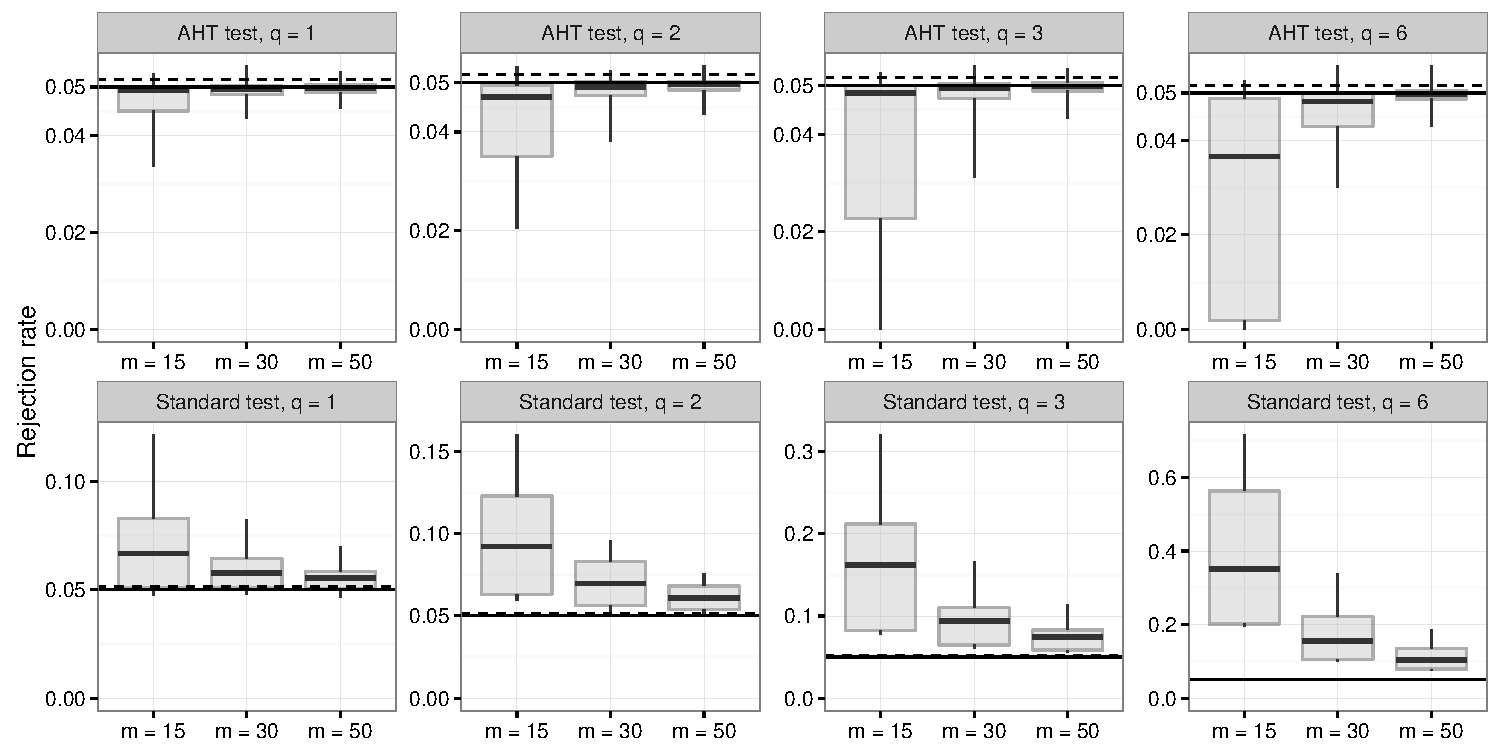
\includegraphics[width=\linewidth]{CR_fig/overview-1} 

}

\caption[Rejection rates of Naive and AHZ tests, by dimension of hypothesis (]{Rejection rates of Naive and AHZ tests, by dimension of hypothesis ($q$) and nominal type I error ($\alpha$)}\label{fig:overview}
\end{sidewaysfigure}


\end{knitrout}

Figure \ref{fig:overview} shows that Naive-F = bad, AHZ = rad! Also, performance of the naive test degrades (becomes liberal) for larger q, whereas AHZ test becomes more conservative.

\begin{knitrout}
\definecolor{shadecolor}{rgb}{0.969, 0.969, 0.969}\color{fgcolor}\begin{sidewaysfigure}

{\centering 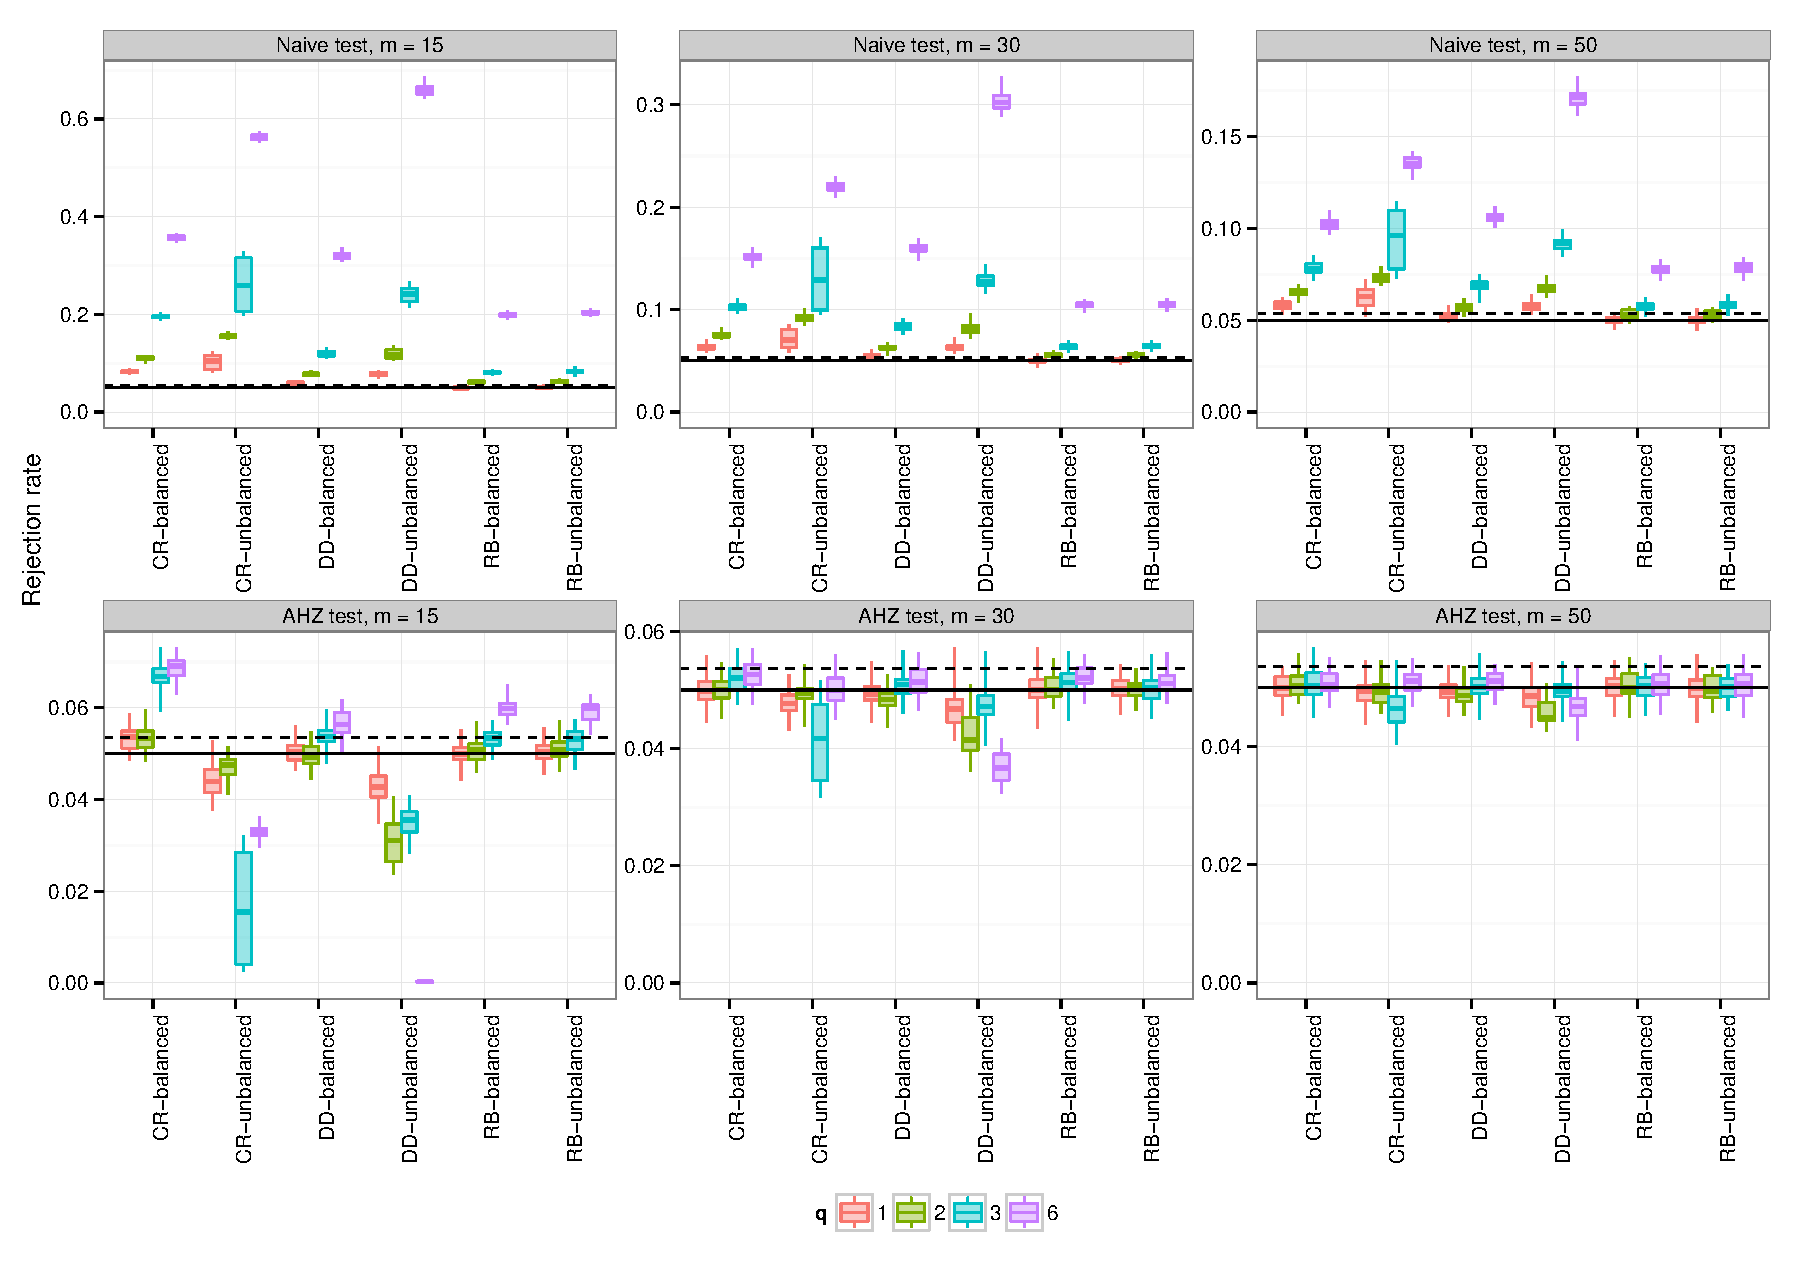
\includegraphics[width=\linewidth]{CR_fig/balance-1} 

}

\caption[Rejection rates of Naive and AHZ tests, by study design and dimension of hypothesis (]{Rejection rates of Naive and AHZ tests, by study design and dimension of hypothesis ($q$). CR = cluster-randomized design; DD = difference-in-differences design; RB = randomized block design.}\label{fig:balance}
\end{sidewaysfigure}


\end{knitrout}

Figure \ref{fig:balance} shows that rejection rates are strongly affected by unbalance of the clusters.

\begin{knitrout}
\definecolor{shadecolor}{rgb}{0.969, 0.969, 0.969}\color{fgcolor}\begin{sidewaysfigure}

{\centering 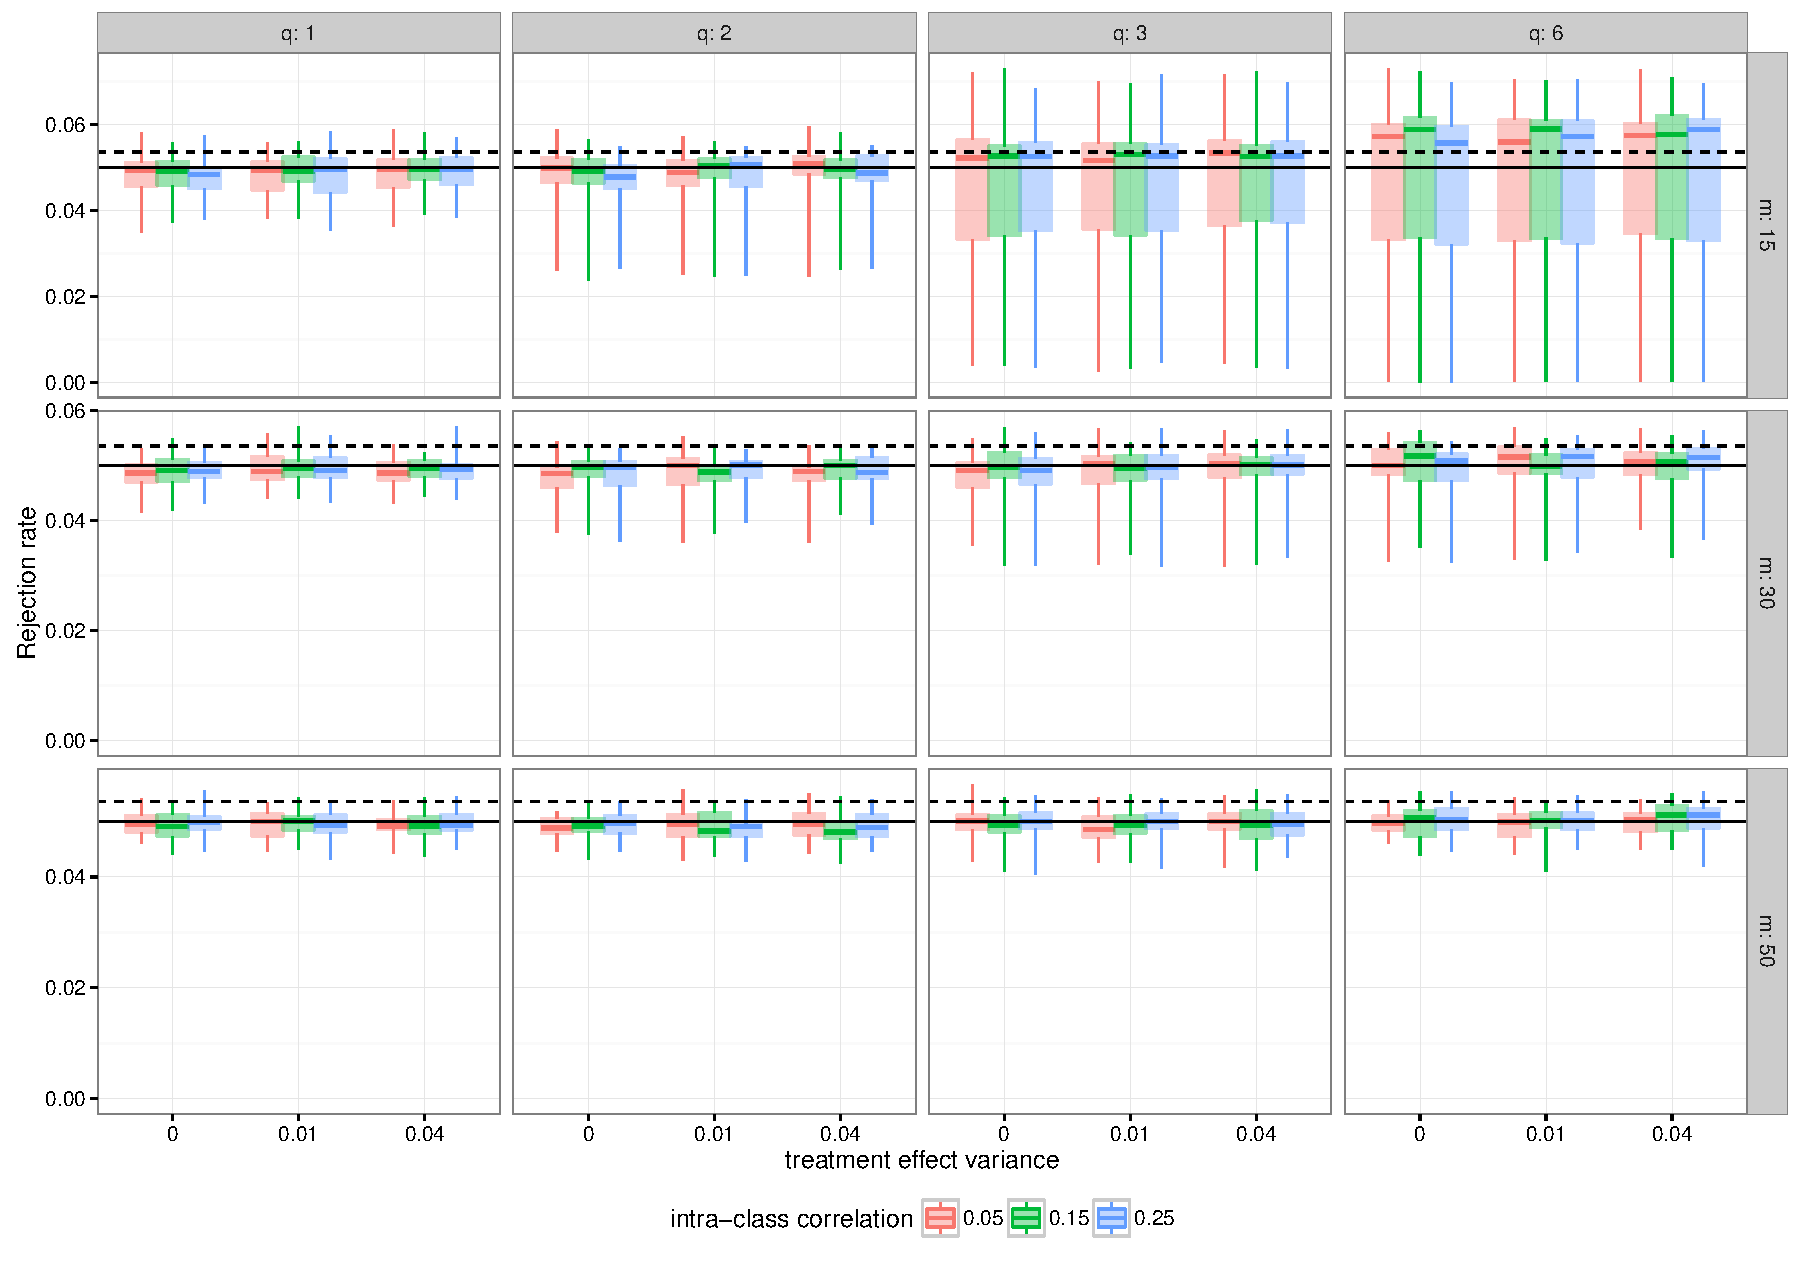
\includegraphics[width=\linewidth]{CR_fig/misspecification-1} 

}

\caption[Rejection rates of AHZ test, by treatment effect variance and intra-class correlation]{Rejection rates of AHZ test, by treatment effect variance and intra-class correlation.}\label{fig:misspecification}
\end{sidewaysfigure}


\end{knitrout}

Figure \ref{fig:misspecification} shows that model mis-specification doesn't matter for AHZ. 

\section{EXAMPLES}
\label{sec:examples}

This section presents three short examples of the use of CRVE with small or moderate samples of clusters, spanning a variety of applied contexts. 
In the first example, the effects of substantive interest are identified within each cluster. 
In the second example, the effects involve between-cluster contrasts. 
The third example involves a cluster-robust Hausmann test for differences between within- and across-cluster information. 
In each example, we demonstrate the proposed small-sample t- and F-tests and compare them to the standard CR1 and Wild bootstrap tests. 
R code and data files are available for each analysis as an online supplement.

\subsection{Tennessee STAR class-size experiment.} 

The Tennessee STAR class size experiment is one of the most intensively studied interventions in education \citep[for a detailed review, see][]{Schanzenbach2006what}.  The experiment involved students in kindergarten through third grade across 79 schools. Within each school, students and their teachers were randomized equally to one of three conditions: small class-size (targetted to have 13-17 students), regular class-size, or regular class-size with an aide.
Among other outcomes, subsequent research has focused on the effects of these conditions on kindergarden reading, math, and word recognition \citep{Achilles2008tennessee}; high school test scores \citep{Schanzenbach2006what}; college entrance exam participation \citep{Krueger2001effect}; and home ownership and earnings \citep{Chetty2011how}.

The STAR experiment involved three treatment conditions and multiple outcomes, providing a scenario where both t-tests (with $q = 1$) and F-tests with varying constraint dimensions can be applied. 
For simplicity, we focus only on the subgroup of students who were in kindergarten during the first year of the study, and on the three outcomes measured at the end of the year, standardized to percentile ranks \citep{Krueger2001effect}: reading, word recognition, and math \citep{Achilles2008tennessee}.
The analytic model is: 
\begin{equation}
y_{ijk} = \bm{r}_{ij}'\bs\beta_k + \bm{s}_{ij}'\bs\gamma_0 + \gamma_k + \mu_i + \epsilon_{ijk}, 
\end{equation}
where $y_{ijk}$ is the percentile rank on outcome $k$ for student $j$ in school $i$; $\bm{r}_{ij}$ includes indicators for the small-class and regular-plus-aide conditions; $\bm{s}_{ij}$ includes student demographic covariates (i.e., free or reduced-price lunch status; race; gender; age); $\gamma_k$ is a fixed effect for outcome $k$; and $\mu_i$ is a fixed effect for school $i$. 
In this model, $\beta_{1k}$ represents the average effect of being in a small class and $\beta_{2k}$ represents the average of effect of being in a regular class with an aid, in each case compared to a regular-size class without an aid.

Using this model, we test four distinct hypotheses that vary in dimension from $q = 1$ to $q = 6$. 
First, using only the data for outcome $k$, we test the effects of small class size ($H_0: \beta_{1k} = 0$) while maintaining the assumption that the additional classroom aide has no effect on student achievement (i.e., constraining $\beta_{2k} = 0$). 
Second, again only using the data for outcome $k$, we test the hypothesis that there are no differences across the three class-size conditions (i.e., $H_0: \bs\beta_k = \bm{0}$). 
Third, combining the data across all three outcomes, we test the hypothesis that small class size (vs regular and regular plus aide) had no effects on any outcome (i.e., $\beta_{11} = \beta_{12} = \beta_{13} = 0$).
Finally, we test the hypothesis that there are no differences across the three class-size conditions on any outcome (i.e., $H_0: \bs\beta_1 = \bs\beta_2 = \bs\beta_3 = \bm{0}$). 
The third and fourth tests use the seemingly unrelated regression (SUR) framework, in which separate treatment effects are estimated for each outcome, but the student demographic effects and school fixed effects are pooled across outcomes. 
In all models, we estimated $\bs\beta_k$ and $\bs\gamma$ after absorbing the school fixed effects and clustering the errors by school.



% latex table generated in R 3.2.3 by xtable 1.8-0 package
% Wed Dec 23 16:20:46 2015
\begin{table}[tbh]
\centering
\begin{tabular}{lllrrr}
  \toprule
Outcome & Effect & Test & F & df & p \\ 
  \midrule
Math & Small class (q=1) & Standard & 13.624 & 78.0 & 0.00041 \\ 
   &  & AHZ & 13.590 & 69.0 & 0.00045 \\ 
   & Small class and classroom aide (q=2) & Standard & 6.838 & 78.0 & 0.00183 \\ 
   &  & AHZ & 6.725 & 68.6 & 0.00215 \\ 
   \midrule
Combined & Small class (q=3) & Standard & 6.408 & 78.0 & 0.00062 \\ 
   &  & AHZ & 6.206 & 67.0 & 0.00088 \\ 
   & Small class and classroom aide (q=6) & Standard & 3.284 & 78.0 & 0.00622 \\ 
   &  & AHZ & 3.042 & 64.9 & 0.01103 \\ 
   \bottomrule
\end{tabular}
\caption{Tests of treatment effects in the Tennessee STAR class size experiment} 
\label{tab:STAR}
\end{table}


Table \ref{tab:STAR} displays the results for a representative subset of these hypothesis tests, using either the standard CR1 hypothesis test or the CR2S test.
These results illustrate two important points regarding the use of the AHZ test in practice.
First, across all three analyses, the CR2 t- and F-tests are typically slightly smaller than those produced using CR1. 
This trend is common, since the BRL adjustments to the variance estimator are typically small in scope.
Second, in the case in which treatment is randomly allocated in equal proportions within each cluster -- as occurs in the TN STAR experiment -- the degrees of freedom for the CR2 tests are only slightly smaller than those for the CR1 tests. 
In combination with the rather large sample size of 79 schools, these differences have only a minimal effect on the p-values for these tests. 
Importantly, these conditions do not always occur in practice, as the next examples will illustrate. 

\subsection{Achievement Awards demonstration} 

\citet{Angrist2009effects} reported results from a randomized trial in Israel that aimed to increase completion rates of the Bagrut, the national matriculation certificate for post-secondary education, among low-achieving high school students. 
In the Achievement Awards demonstration, 40 non-vocational high schools with low rates of Bagrut completion were selected from across Israel, including 10 Arab and 10 Jewish religious schools and 20 Jewish secular schools. 
The schools were then pair-matched based on 1999 rates of Bagrut completion, and within each pair one school was randomized to receive a cash-transfer program. 
In these treatment schools, seniors who completed certification were eligible for payments of approximately \$1,500. 
Student-level covariate and outcome data were drawn from administrative records available for the school years ending in June of 2000, 2001, and 2002. 
The incentive program was in effect for the group of seniors in treatment schools taking the Bagrut exams in Spring of 2001. 
However, the program was discontinued for the following year, and so we treat completion rates for 2000 and 2002 as being unaffected by treatment assignment.
The primary outcome of interest is Bagrut completion. 

This study provides an opportunity to examine the CR2 tests in a situation in which the treatment was assigned at the cluster level, with a smaller number of clusters.
For simplicity, we restrict our analysis to the sample of female students.
Following the original analysis of \citet{Angrist2009effects}, we allow the program's effects to vary depending on whether a students was in the upper or lower half of the distribution of prior-year academic performance. 
Letting $h = 1,2,3$ index the sector of each school (Arab religious, Jewish religious, or Jewish secular), we consider the following analytic model: 
\begin{equation}
\label{eq:AL_ATE}
y_{hitj} = z_{hit}\bm{r}_{hitj}'\bs\beta_h + \bm{s}_{hitj}'\bs\gamma + \gamma_{ht} + \mu_{hi} + \epsilon_{hitj}
\end{equation}
In this model for student $j$ in year $t$ in school $i$ in sector $h$, $z_{hit}$ is an indicator equal to one in the treatment schools for the 2001 school year and otherwise equal to zero; $\bm{r}_{hitj}$ is a vector of indicators for whether the student is in the lower or upper half of the distribution of prior academic performance; and $\bs\beta_h = \left(\beta_{1h}, \beta_{2h}\right)$ is a vector of average treatment effects for schools in sector $h$. 
The vector $\bm{s}_{hitj}$ includes the following individual student demographic measures: mother's and father's education, immigration status, number of siblings, and indicators for each quartile in the distribution of prior-year academic performance. 
The model also includes fixed effects $\gamma_{ht}$ for each sector in each year and $\mu_{hi}$ for each school. 

Based on Model (\ref{eq:AL_ATE}), we test four hypotheses, again with the goal of exploring the use of the CR2S tests in a range of conditions. 
First, we assume that the program effects are constant across sector (i.e., $\bs\beta_1 = \bs\beta_2 = \bs\beta_3 = \bs\beta$) and test for whether the program affected completion rates for students in the upper half of the prior achievement distribution ($H_0: \beta_2 = 0$, with $q = 1$).
Second, we test for whether the program was effective in either half of the prior academic performance ($H_0: \bs\beta = 0$, with $q = 2$), still assuming that program effects are constant across sector. 
Third, we test for whether program effects in the upper half of the prior achievement distribution vary by school sector ($H_0: \beta_{21} = \beta_{22} = \beta_{23}$, with $q = 3$). 
Finally, we conduct a joint test for whether program effects differ across student prior achievement crossed with school sector ($H_0: \bs\beta_1 = \bs\beta_2 = \bs\beta_3$, with $q = 4$). 



% latex table generated in R 3.2.3 by xtable 1.8-0 package
% Wed Dec 23 16:20:47 2015
\begin{table}[bth]
\centering
\begin{tabular}{lcrrr}
  \toprule
Hypothesis & Test & F & df & p \\ 
  \midrule
ATE - upper half (q = 1) & Standard & 5.746 & 34.00 & 0.02217 \\ 
   & AHZ & 5.169 & 15.86 & 0.03726 \\ 
  ATE - joint (q = 2) & Standard & 3.848 & 34.00 & 0.03116 \\ 
   & AHZ & 3.371 & 15.46 & 0.06096 \\ 
   \midrule
Moderation - upper half (q = 2) & Standard & 3.186 & 34.00 & 0.05393 \\ 
   & AHZ & 0.091 & 3.19 & 0.91520 \\ 
  Moderation - joint (q = 4) & Standard & 8.213 & 34.00 & 0.00010 \\ 
   & AHZ & 2.895 & 3.21 & 0.19446 \\ 
   \bottomrule
\end{tabular}
\caption{Tests of treatment effects in the Achievement Awards Demonstration} 
\label{tab:AAD}
\end{table}


Table \ref{tab:AAD} reports the results of all four hypothesis tests. 
These results indicate three important trends.
First, in the case of the first two hypotheses, the CR2 test statistics are only slightly smaller than their CR1 counterparts, though the degrees of freedom are considerably smaller. 
These differences reflect the fact that the treatment indicator occurs at the cluster level, but that the subgroups varied within each cluster. 
Together these lead to a larger impact on results than in the STAR case, where treatment was assigned at the student level.
Second, the third and fourth hypotheses tests -- comparing treatment effects across sectors and subgroups -- illustrates cases in which the CR2S and CR1 tests greatly diverge.
In these cases, the CR2S test statistic and degrees of freedom are both considerably smaller than those from the CR1 test. 
This reflects the degree of unbalance in allocations across sectors (20,10,10) combined with the cluster-level randomization. 
Together these result in cases in which using the small sample adjustments greatly impact the findings. 


% 
% using the CR1 and CR2 adjustments for variance estimation and either the naiv\"e degrees of freedom (for these data, $m - 1 = 34$) or the approximate Hotelling's $T^2$-Z degrees of freedom. 
% Several features of these results are worth noting. 
% First, for the tests of single-parameter hypotheses, the differences between the CR1 and CR2 test statistics are minor, although the AHZ (Satterthwaite) degrees of freedom are substantially lower than the naiv\"e ones. 
% As a result, the $p$-value for the ATE in the upper half of the prior achievement distribution is round(100 * (AL_results[6,"p"] / AL_results[4,"p"] - 1))\% larger based on our preferred test than based on the standard F-test with CR1. 
% Second, the joint test that the ATEs are zero in both halves of the prior achivement distribution is sensitive to both the CR adjustment and the degrees of freedom: the $p$-value based on our preferred test is round(AL_results[9,"p"], 3), compared to the $p = round(AL_results[7,"p"], 3)$ for the standard test. 
% Finally, the test of moderation by sector is strongly affected by the CR2 adjustment and AHZ degrees of freedom. 
% In particular, the AHZ degrees of freedom are just round(AL_results[12,"df"],2), far lower than the number of clusters. 
% The low degrees of freedom are a consequence of the small number of schools of each type in each treatment condition.
% Although the total sample includes 35 schools, there are only 9 Arab religious, 7 Jewish religious, and 19 Jewish secular schools, each split across two treatment conditions, and the treatment effects are estimated by making comparisons across clusters. 
% As a result, the F statistic based on CR2 has a very large sampling variance under the null hypothesis.
% \todo{Connect to simulation results--higher $q$, between-cluster}

\subsection{Effects of minimum legal drinking age on mortality} 

In this final example, we shift focus from analyses of experiments to panel data, using an example described in Angrist and Pischke (2015)\todo{Cite}.
Using data from the Fatal Accident Reporting System maintained by the National Highway Traffic Safety Administration, we examine the effects of changes in the minimum legal drinking age over the time period of 1970-1983 on state-level death rates resulting from motor vehicle crashes.\todo{Note about measure of legal drinking age.}
A standard difference-in-differences specification for such a state-by-year panel is
\begin{equation}
\label{eq:MLDA}
y_{it} = \bm{r}_{it}'\bs\beta + \gamma_t + \mu_i + \epsilon_{it}.
\end{equation}
In this model, time-point $t$ is nested within state $i$; the outcome $y_{it}$ is the number of deaths in motor vehicle crashes (per 100,000 residents) in state $i$ at time $t$; $\bm{r}_{it}$ is a vector of covariates; $\gamma_t$ is a fixed effect for time point $t$; and $\mu_i$ is an effect for state $i$. The vector $\bm{r}_{it}$ consists of a measure of the proportion of the population between the ages of 18 and 20 years who can legally drink alcohol and a measure of the beer taxation rate, both of which vary across states and across time.. 

In order to estimate the effect of lowering the legal drinking age, we apply both random effects (RE) and fixed effects (FE) estimation. 
For the RE estimates, we use WLS with weights derived under the assumption that  $\mu_1,...,\mu_m$ are mutually independent, normally distributed, and independent of $\epsilon_{it}$.
We also report an artificial Hausman test \citep{Arellano1993on, Wooldridge2002econometric} for correlation between the covariates $\bm{r}_{it}$ and the state effects $\mu_i$. Such correlation creates bias in the RE estimator of the policy effect, thus necessitating the use of the FE estimator.
The artificial Hausman test amends model (\ref{eq:MLDA}) to include within-cluster deviations (or cluster aggregates) of the variables of interest, so that the estimating equation is
\begin{equation}
y_{it} = \bm{r}_{it}\beta + \bm{\ddot{r}}_{it}\bs\delta + \gamma_t + \mu_i + \epsilon_{it},
\end{equation}
where $\bm{\ddot{r}}_{it}$ denotes the within-cluster deviations of the covariate.
The parameter $\bs\delta$ captures the difference between the between-panel and within-panel estimates of $\bs\beta$. 
With this setup, the artificial Hausmann test amounts to testing the null hypothesis that $\bs\delta = \bm{0}$, where $\bs\delta$ is estimated using RE.  



% latex table generated in R 3.2.3 by xtable 1.8-0 package
% Wed Dec 23 16:20:47 2015
\begin{table}[bth]
\centering
\begin{tabular}{lcrrr}
  \toprule
Hypothesis & Test & F & df & p \\ 
  \midrule
Random effects & Standard & 8.261 & 49.00 & 0.00598 \\ 
   & AHZ & 7.785 & 24.74 & 0.00999 \\ 
  Fixed effects & Standard & 9.660 & 49.00 & 0.00313 \\ 
   & AHZ & 9.116 & 22.72 & 0.00616 \\ 
   \midrule
Hausman test & Standard & 2.930 & 49.00 & 0.06283 \\ 
   & AHZ & 2.489 & 8.69 & 0.13980 \\ 
   \bottomrule
\end{tabular}
\caption{Tests of effects of minimum legal drink age and Hausman specification test} 
\label{tab:MLDA}
\end{table}


Table \ref{tab:MLDA} displays the results of the tests for the policy variable and the Hausman tests for each model specification. 
As in previous examples, our preferred version of the test uses the CR2S adjustment to the variance estimator and the AHZ test. 
The results of the policy effect tests are quite similar across specifications and versions of the test. 
Of note is that the RE and FE estimates have only half the degrees of freedom of the naiv\"e test. 
For the artificial Hausman test the AHZ test has fewer than 9 degrees of freedom, which leads to a much larger p-value compared to using the CR1 F test. 

\section{DISCUSSION}
\label{sec:discussion}

Cluster robust standard errors are common practice in economic applications, since in large samples they require few assumptions regarding the error structure of the data.
In small and moderate samples, however, the CRVE approach can result in overly liberal tests, with Type I error far above nominal.
A promising solution therefore is to incorporate a working model for the error structure into the CRVE approach -- bias reduced linearization -- as introduced by Bell and McCaffrey (2002), and to use estimated degrees of freedom.
In this paper, we have provided solutions to three problems facing the implementation of this BRL approach in economics, making the method useful in a wide range of applications.

While the idea of identifying and implementing a working model for the error structure seems antithetical to the idea of CRVE, simulations studies provided here and elsewhere show that the approach is robust to a high degree of misspecification of this working model.
Importantly, the role of this structure while larger when the number of clusters is very small, effectively falls away as the number of clusters increases, converging to the usual CRVE estimator in large samples.
This structure greatly improves the performance of CRVE, bringing the Type I error in line with the stated $\alpha$ levels for tests, even in less than ideal situations.

The main driver to these adjustments, as illustrated both in the simulation study and the set of examples, is the fact that in this approach the degrees of freedom are estimated using a Satterthwaite approximation.
These degrees of freedom can be much smaller than the number of clusters, particularly when the covariates being tested exhibit a high degree of unbalance or skewness.
In economics, these problems are common, particularly in the analysis of experiments and in difference-in-difference models used in panel data. 
In this paper, we have shown that the small sample adjustments provided here perform well even in situations in which a series of policies are allocated very unequally across groups, and that the approach works by greatly reducing the degrees of freedom.
In many cases these degrees of freedom can be quite small, even when the number of clusters is moderate to large.
Most striking, perhaps, is the fact that these differences occur even with as many as 50 clusters, a rule of thumb often given for when CRVE should perform well.


%Current take-home points:
%\begin{itemize}
%\item How much does the working matrix matter?
%\item Role of degrees of freedom
%\item Logical consistency: t-test and F-test; FE and absorbtion
%\item Comparing these to CR1
%\item Comparing these to Wild bootstrap
%\item Previous research has broken out CR* from the test. We didn't do this this time because...


%Future research:
%\begin{itemize}
%\item ``empirical'' degrees of freedom estimation
%\item use of other CR estimators
%\item computational issues with CR2 (especially when $n_i$'s are large)
%\item saddlepoint methods for $q > 1$
%\end{itemize}

\appendix

\section{BRL adjustment matrices}
\label{app:theorems}

This appendix provides proof of the two theorems from Section \ref{sec:BRL}. 

\subsection{Proof of Theorem \ref{thm:BRL_FE}}

The Moore-Penrose inverse of $\bm{B}_i$ can be computed from its eigen-decomposition. Let $b \leq n_i$ denote the rank of $\bm{B}_i$. 
Let $\bs\Lambda$ be the $b \times b$ diagonal matrix of the positive eigenvalues of $\bm{B}_i$ and $\bm{V}$ be the $n_i \times b$ matrix of corresponding eigen-vectors, so that $\bm{B}_i = \bm{V}\bs\Lambda\bm{V}'$. 
Then $\bm{B}_i^+ = \bm{V}\bs\Lambda^{-1}\bm{V}'$ and $\bm{B}_i^{+1/2} = \bm{V}\bs\Lambda^{-1/2}\bm{V}'$. Now, observe that 
\begin{align}
\label{eq:step1}
\bm{\ddot{R}}_i' \bm{W}_i \bm{A}_i \left(\bm{I} - \bm{H_X}\right)_i \bs\Phi \left(\bm{I} - \bm{H_X}\right)_i' \bm{A}_i' \bm{W}_i \bm{\ddot{R}}_i &= \bm{\ddot{R}}_i' \bm{W}_i \bm{D}_i \bm{B}_i^{+1/2} \bm{B}_i \bm{B}_i^{+1/2} \bm{D}_i' \bm{W}_i \bm{\ddot{R}}_i \nonumber \\
&= \bm{\ddot{R}}_i' \bm{W}_i \bm{D}_i \bm{V}\bm{V}' \bm{D}_i' \bm{W}_i \bm{\ddot{R}}_i. 
\end{align}

Because $\bm{D}_i$, and $\bs\Phi$ are positive definite and $\bm{B}_i$ is symmetric, the eigenvectors $\bm{V}$ define an orthonormal basis for the column span of $\left(\bm{I} - \bm{H_{\ddot{X}}}\right)_i$.
We now show that $\bm{\ddot{U}}_i$ is in the column space of $\left(\bm{I} - \bm{H_X}\right)_i$. 
Let $\bm{Z}_i$ be an $n_i \times (r + s)$ matrix of zeros. 
Let $\bm{Z}_k = - \bm{\ddot{U}}_k \bm{L}^{-1}\bm{M}_{\bm{\ddot{U}}}^{-1}$, for $k \neq j$ and take $\bm{Z} = \left(\bm{Z}_1',...,\bm{Z}_m'\right)'$. 
Now observe that $\left(\bm{I} - \bm{H_T}\right) \bm{Z} = \bm{Z}$. 
It follows that 
\begin{align*}
\left(\bm{I} - \bm{H_X}\right)_i \bm{Z} &= \left(\bm{I} - \bm{H_{\ddot{U}}}\right)_i \left(\bm{I} - \bm{H_T}\right) \bm{Z} = \left(\bm{I} - \bm{H_{\ddot{U}}}\right)_i \bm{Z} \\
&= \bm{Z}_i - \bm{\ddot{U}}_i\bm{M_{\ddot{U}}}\sum_{k=1}^m \bm{\ddot{U}}_k'\bm{W}_k\bm{Z}_k = \bm{\ddot{U}}_i\bm{M_{\ddot{U}}} \left(\sum_{k \neq j} \bm{\ddot{U}}_k' \bm{W}_k \bm{\ddot{U}} \right) \bm{L}^{-1}\bm{M}_{\bm{\ddot{U}}}^{-1} \\
&= \bm{\ddot{U}}_i.
\end{align*}
Thus, there exists an $N \times (r + s)$ matrix $\bm{Z}$ such that $\left(\bm{I} - \bm{H_{\ddot{X}}}\right)_i \bm{Z} = \bm{\ddot{U}}_i$, i.e., $\bm{\ddot{U}}_i$ is in the column span of $\left(\bm{I} - \bm{H_X}\right)_i$. Because $\bm{D}_i \bm{W}_i$ is positive definite and $\bm{\ddot{R}}_i$ is a sub-matrix of $\bm{\ddot{U}}_i$, $\bm{D}_i\bm{W}_i\bm{\ddot{R}}_i$ is also in the column span of $\left(\bm{I} - \bm{H_X}\right)_i$. It follows that 
\begin{equation}
\label{eq:step2}
\bm{\ddot{R}}_i' \bm{W}_i \bm{D}_i \bm{V}\bm{V}' \bm{D}_i' \bm{W}_i \bm{\ddot{R}}_i = \bm{\ddot{R}}_i' \bm{W}_i \bs\Phi_i \bm{W}_i \bm{\ddot{R}}_i.
\end{equation}
Substituting (\ref{eq:step2}) into (\ref{eq:step1}) demonstrates that $\bm{A}_i$ satisfies criterion (\ref{eq:CR2_criterion}).

Under the working model, the residuals from cluster $i$ have mean $\bm{0}$ and variance \[
\Var\left(\bm{\ddot{e}}_i\right) = \left(\bm{I} - \bm{H_X}\right)_i \bs\Phi \left(\bm{I} - \bm{H_X}\right)_i',\] 
It follows that 
\begin{align*}
\E\left(\bm{V}^{CR2}\right) &= \bm{M_{\ddot{R}}}\left[\sum_{i=1}^m \bm{\ddot{R}}_i' \bm{W}_i \bm{A}_i \left(\bm{I} - \bm{H_X}\right)_i \bs\Phi \left(\bm{I} - \bm{H_X}\right)_i' \bm{A}_i \bm{W}_i \bm{\ddot{R}}_i \right] \bm{M_{\ddot{R}}} \\
&= \bm{M_{\ddot{R}}}\left[\sum_{i=1}^m \bm{\ddot{R}}_i' \bm{W}_i \bs\Phi_i \bm{W}_i \bm{\ddot{R}}_i \right] \bm{M_{\ddot{R}}} \\
&= \Var\left(\bs{\hat\beta}\right)
\end{align*}

\subsection{Proof of Theorem \ref{thm:absorb}}

From the fact that $\bm{\ddot{U}}_i'\bm{W}_i\bm{T}_i = \bm{0}$ for $i = 1,...,m$, it follows that \begin{align*}
\bm{B}_i &= \bm{D}_i \left(\bm{I} - \bm{H_{\ddot{U}}}\right)_i \left(\bm{I} - \bm{H_T}\right) \bs\Phi \left(\bm{I} - \bm{H_T}\right)' \left(\bm{I} - \bm{H_{\ddot{U}}}\right)_i' \bm{D}_i'\\
&= \bm{D}_i \left(\bm{I} - \bm{H_{\ddot{U}}} - \bm{H_T}\right)_i \bs\Phi \left(\bm{I} - \bm{H_{\ddot{U}}} - \bm{H_T}\right)_i' \bm{D}_i' \\
&= \bm{D}_i \left(\bs\Phi_i - \bm{\ddot{U}}_i \bm{M_{\ddot{U}}}\bm{\ddot{U}}_i' - \bm{T}_i \bm{M_T}\bm{T}_i'\right)\bm{D}_i'
\end{align*}
and 
\begin{equation}
\label{eq:B_i_inverse}
\bm{B}_i^+ = \left(\bm{D}_i'\right)^{-1} \left(\bs\Phi_i - \bm{\ddot{U}}_i \bm{M_{\ddot{U}}}\bm{\ddot{U}}_i' - \bm{T}_i \bm{M_T}\bm{T}_i'\right)^+ \bm{D}_i^{-1}.
\end{equation}
Let $\bs\Psi_i = \left(\bs\Phi_i - \bm{\ddot{U}}_i \bm{M_{\ddot{U}}}\bm{\ddot{U}}_i'\right)^+$.
Using a generalized Woodbury identity \citep{Henderson1981on}, \[
\bs\Psi_i = \bm{W}_i + \bm{W}_i \bm{\ddot{U}}_i \bm{M_{\ddot{U}}}\left(\bm{M_{\ddot{U}}} - \bm{M_{\ddot{U}}} \bm{\ddot{U}}_i' \bm{W}_i \bm{\ddot{U}}_i \bm{M_{\ddot{U}}}\right)^+ \bm{M_{\ddot{U}}}\bm{\ddot{U}}_i'\bm{W}_i. \]
It follows that $\bs\Psi_i \bm{T}_i = \bm{W}_i \bm{T}_i$. 
Another application of the generalized Woodbury identity gives 
\begin{align*}
\left(\bs\Phi_i - \bm{\ddot{U}}_i \bm{M_{\ddot{U}}}\bm{\ddot{U}}_i' - \bm{T}_i \bm{M_T}\bm{T}_i'\right)^+ &= \bs\Psi_i + \bs\Psi_i \bm{T}_i \bm{M_T}\left(\bm{M_T} - \bm{M_T}\bm{T}_i' \bs\Psi_i \bm{T}_i \bm{M_T}\right)^+ \bm{M_T} \bm{T}_i' \bs\Psi_i \\
&= \bs\Psi_i + \bm{W}_i \bm{T}_i \bm{M_T}\left(\bm{M_T} - \bm{M_T}\bm{T}_i' \bm{W}_i \bm{T}_i\bm{M_T}\right)^+ \bm{M_T} \bm{T}_i' \bm{W}_i \\
&= \bs\Psi_i.
\end{align*}
The last equality follows from the fact that $\bm{T}_i \bm{M_T}\left(\bm{M_T} - \bm{M_T}\bm{T}_i' \bm{W}_i \bm{T}_i\bm{M_T}\right)^{-} \bm{M_T} \bm{T}_i' = \bm{0}$ because the fixed effects are nested within clusters. 
Substituting into (\ref{eq:B_i_inverse}), we then have that $\bm{B}_i^+ = \left(\bm{D}_i'\right)^{-1} \bs\Psi_i \bm{D}_i^{-1}$. 
But \[
\bm{\tilde{B}}_i = \bm{D}_i \left(\bm{I} - \bm{H_{\ddot{U}}}\right)_i \bs\Phi \left(\bm{I} - \bm{H_{\ddot{U}}}\right)_i' \bm{D}_i' = \bm{D}_i \left(\bs\Phi_i - \bm{\ddot{U}}_i\bm{M_{\ddot{U}}} \bm{\ddot{U}}_i'\right) \bm{D}_i' = \bm{D}_i \bs\Psi_i^+ \bm{D}_i',
\]
and so $\bm{B}_i^+ = \bm{\tilde{B}}_i^+$. It follows that $\bm{A}_i = \bm{\tilde{A}}_i$ for $i = 1,...,m$. 

\bibliographystyle{agsm}
\bibliography{bibliography}

\end{document}

